\section{Introduction}

\subsection{Motivation}
In the mathematical literature, many authors have considered models to modelling the evolution of a population under the effect of mutations. In 1930, Fisher models the invasion of a mutant in a given population by the reaction-diffusion equation
    \begin{equation*}
        \partial_t u - \Delta u = u(1-u)
        \eqfinv
    \end{equation*} 
where $u$ represents the density of the mutant in the population. \ndr{preciser le terme density ? }. 
Since then, diffusion-reaction models have been widely studied to understand mutation phenomena \cite{alfaro2017replicator,alfaro2017superexponential}. 
These models were then extended to a non-local variant where the diffusion is replaced by a convolution operator \cite{coville2007non} and an integral operator \cite{burger1996stationary,bonnefon2015concentration}. \\

In~\cite{robert2018mutation}, the authors have considered a microfluidic setting to study the impact of a new mutation on the fitness of a cell. 
In this setting, they consider a population of cells $u(t,x)$ evolving through the time $t \in \RR_+$ and structured by the growth rate $x \in \RR_+$. Mutations are assumed to happen at a constant rate $\mu$ which is justified by biological experiments \cite{robert2018mutation}.  Assume that $k(x,y)\diff t$ is the fraction of individuals with a growth rate $y$ evolving towards a growth rate $x$ under the effect of mutation during the time interval $\diff t$. The model may be written as \ndr{Mal dit}
    \begin{equation}
    \f{\partial}{\partial t} u(t,x) = - \mu u(t,x) + \mu \int\limits_0^\infty k(x,y) u(y) \diff y 
    \eqfinp
    \label{eq:lydia}
    \end{equation}

Apart from its biological interest, we note that Equation~\eqref{eq:lydia} is very similar to the fragmentation equation which has many applications. Only a few reference are given here among the huge number of applications : aggregation of proteins \cite{xue2013imaging}, cell division \cite{doumic2013estimating}, mining industry \cite{kolmogorov1941logarithmic, bertoin2005fragmentation}, polymer degradation \cite{montroll1940theory,ziff1985kinetics}. \\

In this article, we assume that $k(x,y) := \f{1}{y}k \big(\frac{x}{y}\big)$, which leads to the equation
\begin{equation}
    \f{\partial}{\partial t} u(t,x) = - \mu u(t,x) + \mu \int\limits_0^\infty k\left(\frac{x}{y}\right) u(y) \f{\diff y}{y} 
    \eqfinp
    \label{eq:lydia_selfsimilar}
\end{equation}
This assumption is referred as the \textit{'self-similarity property'}. It reflects the fact that the probability to obtain a cell of fitness $y$ out of a particle of size $x$ only depends on the ration $y/x$. This is a classical assumption for the fragmentation equation \ndr{ref ?} which is related to the mutation equation. \\
    
We aim to understand the asymptotic behavior of $u$ when $t \to \infty$. We want to understand how the distribution of mutants evolves over time, first in a population that is not growing, then in a growing population. If the fitness of the mutants increases indefinitely, we would like to be able to characterise an escape rate. Conversely, if all the mutants die, we would like to obtain a population collapse rate. \ndr{Mal dit... à refaire}
    
\subsection{Review on existing results} Many authors have studied mutation-selection models. 
In \cite{burger1996stationary}, the authors study a model close to Equation~$\eqref{eq:lydia_selfsimilar}$ where they have a bounded growth coefficient.  They prove the existence and uniqueness of a solution for the Cauchy problem by using semigroup theory.
In \cite{eshel1972evolution}, the author assume that each mutation are equi-distributed around the parental type in a discrete time setting. \\ 
    
When all mutations are deleterious, the support of $k$ is contained in $(0,1)$. In this case, Equation~\eqref{eq:lydia_selfsimilar} is known as the fragmentation equation for which many studies have already be done: existence and uniqueness for the Cauchy problem \cite{melzak1957scalar}, asymptotic behaviour \cite{doumic2016time}, reconstructing the kernel of fragmentation \cite{hoang2017estimating,hoang2017nonparametric, doumic2018estimating,doumic2021inverse}, when the size of particles is modified by fragmentation and diffusion at a constant rate \cite{laurenccot2022fragmentation}. 
For a rather complete list of references the reader may consult \cite{banasiak2019analytic,bertoin2006random}.
    

\subsection{Main results and organization of the article} In the present article, 

In Section~\ref{}
In Section~\ref{}, we seek to see if the growth of the population may compensate the effect of deleterious mutations. 

To summarize, the main novelties brought by this article are: 
\begin{itemize}
    \item An extension of the work done in \cite{doumic2016time} when the support of $k \subset (0, \infty)$
    \item 
\end{itemize}

The organization of the article is as follows.

\subsection{Notation}

Let $\Ccal(\RR_+)$ be the set of continuous functions on $\RR_+$. We define the supremum norm
\begin{equation*}
    \|\varphi\|_{\infty} :=\sup_{x \in \RR_+} \left\{ |\varphi(x)| \right\}
    \eqfinp
\end{equation*}

The set $\Mcal(\RR_+)$ is the set of Radon measures $\mu$ such that $\supp(\mu) \subset \RR_+$. The TV--norm of a measure $\mu \in \Mcal(\RR_+)$ is given by 
    \begin{equation*}
        \|\mu\|_{TV} :=\sup \left\{ \int_{\RR_+} \varphi(x) \mu(\dd x)\; ; \; \varphi \in \Ccal(\RR_+)\cap L^1(\dd|\mu|),\; \|\varphi\|_{\infty} \leq 1\right\}
    \end{equation*}
We recall that $\left(\Mcal(\RR_+), \|\cdot\|_{TV}\right)$ is a Banach space. 


\section{The Mutation Equation : mutation can be deleterious or beneficial}

\subsection{Location of the population}

Consider the equation
\begin{equation}\left\{
    \begin{array}{ll}
	\frac{\partial}{\partial t}u(t,x) = - \mu u(t,x) + \mu \int_{0}^{\infty} k\big( \frac{x}{y}\big)u(t,y) \frac{\dy}{y}
	\eqsepv
	& t \in (0, \infty), x \in \RR_+, \mu \in (0, \infty) \eqfinv
	\\
	u(0, x) = u_0(x)
	& x \in \RR_+
	\eqfinp
    \end{array}
	\right.
    \label{eq:main}
\end{equation}

We assume that the initial data $u_0(x)$ is a function satisfying the following conditions 
$$ u_0 \geq 0 \eqsepv \int_0^\infty u_0(x)(1+x)\diff x < \infty.$$
It follows that the Mellin transform of $u_0$, $U_0(s)= \int_0^\infty x^{s-1}u(t,x)\diff x$ is analytic on the strip $\Re(\alpha) \in (p_0,q_0)$ where $p_0 \leq 1 < 2 \leq q_0$ \\
For the simplicity, we assume that 
$ p_0=-\infty$ and $q_0 = \infty$\\

By applying the Mellin transform for Equation~\eqref{eq:main}, we have
	\begin{equation}
		\frac{\partial}{\partial t} U(t,s) = - \mu U(t,s) + \mu K(s) U(t,s)
		\eqfinp
        \label{eq:explicit_reconstruction}
	\end{equation}
If we have some good hypothesis (see Section~\ref{s:explicit}) on $U_0$ and $K$, then we have an explicit formula for the inverse Mellin transform and it follows that
    \begin{equation*}
        U(t,s) = U_0(s) e^{-\mu t(1 - K(s) ) }
        \eqsepv
        U_0(s) = \Mcal_{u_0}(s)
        \eqfinp
    \end{equation*}

Here, $K$ is a convex function, such that $K(1) = 1$. We denote $s_* = \argmin_{s\in \RR} K(s)$. 

\subsection{Examples of kernel}

\textit{1.} $k_0(x) = \delta_\alpha$ \\
\textit{2.} $k_0(x) = \frac{1}{b-a}\1{(a,b)}$, $a,b > 0$ \\
Then for all $s \neq 0$, 
    \begin{align*}
        K(s) = \frac{1}{b-a}\int_a^b x^{s-1}\diff x = \frac1s \cdot\frac{b^s - a^s}{b-a}
        \eqfinp
    \end{align*}
\textit{3. The Log--normal kernel.} $k_0(x) = \frac{1}{\sqrt{2\pi}\sigma x} e^{-\frac{(\log(x)-m)^2}{2\sigma^2}}$.
By the change of variables $y = \log(x)$, we have
    \begin{align*}
        K(s) 
        &= \int_0^\infty \frac{x^{s-2}}{\sqrt{2\pi}\sigma} e^{-\frac{(\log(x)-m)^2}{2\sigma^2}} \diff x \\
        &= \int_{-\infty}^\infty \frac{e^{y(s-1)}}{\sqrt{2\pi}\sigma} e^{-\frac{(y-m)^2}{2\sigma^2}} \diff y \\
        &=  \int_{-\infty}^\infty \frac{1}{\sqrt{2\pi}\sigma} e^{\frac{-y^2 - m^2 + 2m y + 2\sigma^2 y(s-1)}{2\sigma^2}} \diff y \\
        &=  \int_{-\infty}^\infty \frac{1}{\sqrt{2\pi}\sigma} e^{\frac{-y^2 - m^2 + 2y[m + \sigma^2 (s-1)]}{2\sigma^2}} \diff y \\
        &=  \int_{-\infty}^\infty \frac{1}{\sqrt{2\pi}\sigma} 
        e^{-\frac{(y - [m + \sigma^2 (s-1)])^2}{2\sigma^2}}
        e^{\frac{2m \sigma^2(s-1)+\sigma^4(s-1)^2}{2\sigma^2}}\diff y \\
        &=  \int_{-\infty}^\infty \frac{1}{\sqrt{2\pi}\sigma} 
        e^{-\frac{(y - [m + \sigma^2 (s-1)])^2}{2\sigma^2}}
        e^{m (s-1)+\frac{\sigma^2}{2}(s-1)^2}\diff y
        \eqfinp
    \end{align*}
Let denote $  := e^{m (s-1)+\frac{\sigma^2}{2}(s-1)^2}$, then 
\begin{align*}
    K(s) 
    &=  C(s,m,\sigma) \int_{-\infty}^\infty \frac{1}{\sqrt{2\pi}\sigma} 
        e^{-\frac{(y - [m + \sigma^2 (s-1)])^2}{2\sigma^2}}\diff y
        \\
        &=  \frac{C(s,m,\sigma)}{\sqrt{2\pi}\sigma} \int_{-\infty}^\infty
        e^{-\frac{(y - [m + \sigma^2 (s-1)])^2}{2\sigma^2}}\diff y
\end{align*}



\subsection{A first lemma}

\begin{lemma}Let $k_0$ be a positive measure on $\RR_+$ and $K(s):\RR \to [0,+\infty]$ given by $$K(s)=\int_0^\infty x^{s-1}k_0(\diff x)$$ its Mellin transform. We note $<p_0,q_0>$the fundamental strip of $K$.
\begin{enumerate}
    \item If $K$ is strictly decreasing, then $q_0 = \infty$ and  $\supp k_0 \subset [0,1]$.
    \item If $K$ is strictly increasing, then $p_0 = -\infty$ and $\supp k_0 \subset [1, \infty]$.
\end{enumerate}
\end{lemma}
\begin{proof}
\textit{2st case}: If $K$ is strictly increasing, then $K(s)<K(1)$ for all $s < 1$.


For any $s \in (-\infty, q_0)$, we have
\begin{align*}
    K(s) = \int_0^1 x^{s-1} k_0(\diff x) + \int_1^\infty x^{s-1} k_0(\diff x)
\end{align*}
where these two integrals exist because the integrands are positives and that the integrals are bounded by $K(s)$. \\

Assume there exist a measurable set $A \in \Bcal(\RR_+) \cap (0,1-\varepsilon)$ for some $0 < \varepsilon < 1$ such that $k_0(A) > 0$.  It follows that 
\begin{align*}
   K(1) > K(s) > \int_A x^{s-1} k_0(\diff x)
   > (1-\varepsilon)^{s-1} k_0(A)
   \,,\quad \forall s < 1
   \eqfinp
\end{align*}
But $$(1-\varepsilon)^{s-1} k_0(A) \to \infty \mtext{as} s \to -\infty$$
It's absurd. Therefore for all measurable sets $A \subset (0,1-\varepsilon)$, $k_0(A) = 0$. It follows that  
$$\forall A \in \Bcal\big((0,1)\big), k_0(A) = 0.$$
Therefore, $\supp(k_0) \subset [1, \infty]$.
\end{proof}

The next proposition shows that the behaviour of the repartition of the population depends on $s_* < 1$ or $s_* > 1$. 
\begin{figure}
    \centering
    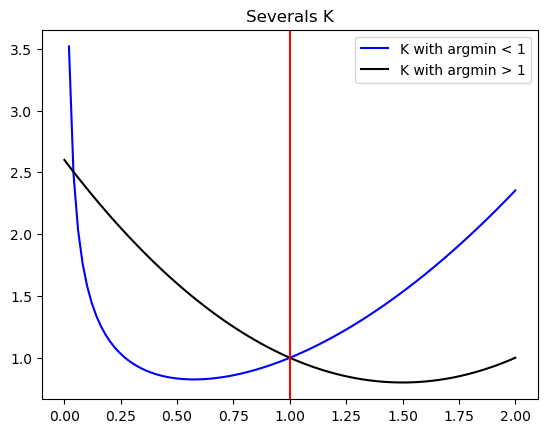
\includegraphics[scale=0.8]{pictures/severalK.png}
    \caption{The Mellin transform $K(s)$ for two kernel $k_0$. The red point shows the minimum of $K$ }
    \label{fig:severalK}
\end{figure}

\begin{proposition} Let $R>0$.
    \begin{enumerate}
        \item Suppose that $s_* < 1$, then
            \begin{align*}
            \lim_{t\to \infty} \int_R^\infty u(t,x) \diff x = \int_0^\infty u_0(x) \diff x
            \eqfinp
            \end{align*}
        \item Suppose that $s_* > 1$, then
            \begin{align*}
            \lim_{t\to \infty} \int_0^R u(t,x) \diff x = \int_0^\infty u_0(x) \diff x
            \eqfinp
            \end{align*}
    \end{enumerate}
\end{proposition}

\begin{proof}\text{}\\

\textbf{First case:} Suppose that $s_* < 1$. Let $c$ be a real $>1$. 
By Mellin inversion, we have that
\begin{align*}
    u(t,x) = \frac{1}{2i\pi}\int_{c-i\infty}^{c+i\infty} U_0(s) x^{-s} e^{-\mu t(1 - K(s))} \diff s
\end{align*}

It follows that
\begin{align*}
    \int_R^\infty u(t,x) \diff x 
    &= \frac{1}{2i\pi} \int_R^\infty \int_{c-i\infty}^{c+i\infty} U_0(s) x^{-s} e^{-\mu t(1 - K(s))} \diff s \diff x \\
    &= \frac{1}{2i\pi} \int_{c-i\infty}^{c+i\infty} \int_R^\infty U_0(s) x^{-s} e^{-\mu t(1 - K(s))} \diff x \diff s \\
    &= \frac{1}{2i\pi} \int_{c-i\infty}^{c+i\infty} U_0(s) \frac{R^{-s+1}}{s-1} e^{-\mu t(1 - K(s))} \diff s \\
    &= \frac{1}{2i\pi} \int_{c-i\infty}^{c+i\infty}\frac{U_0(s)}{s-1} e^{-\mu t(1 - K(s))} e^{(-s+1)\ln R} \diff s 
\end{align*}
(The exchange between the two integrals come from the fact that $c > 1$.)

We deform the integration contour towards the left and cross the pole $s = 1$. The Cauchy's residue theorem ensures that
\begin{align}
    \int_R^\infty u(t,x) \diff x &= \mathrm{Res(1)} + \frac{1}{2i\pi} \int_{s_*-i\infty}^{s_*+i\infty} \frac{U_0(s)}{s-1} e^{-\mu t(1 - K(s))} e^{(-s+1)\ln R} \diff s
    \label{eq:cauchy1}
\end{align}

We define
\begin{align*}
    \Rcal(t) = \frac{1}{2i\pi} \int_{s_*-i\infty}^{s_*+i\infty} \frac{U_0(s)}{s-1} e^{-\mu t(1 - K(s))} e^{(-s+1)\ln R} \diff s
    \eqfinp
\end{align*}
We have 
\begin{align*}
    |\Rcal(t)| 
    &\leq \frac{R^{1-s_*}}{2\pi} \int_{s_*-i\infty}^{s_*+i\infty} \left|\frac{U_0(s) }{s-1}\right| \cdot \left|e^{-\mu t(1 - K(s))}\right| \diff s \\
    &= \frac{R^{1-s_*}}{2\pi} \int_{s_*-i\infty}^{s_*+i\infty} \left|\frac{U_0(s) }{s-1}\right| e^{\Re[-\mu t(1 - K(s))]} \diff s
    \eqfinp
\end{align*}
However, for all $s = s_* + i\nu \in (s_*-i \infty, s_* + i \infty)$
\begin{align*}
    \Re[-\mu t(1 - K(s))] 
    &= \Re[-\mu t(K(1) - K(s))] \\
    &= -\mu t \Re\left( K(1) - \int_0^\infty z^{s-1}k_0(z)\diff z  \right) \\
    &=  -\mu t\left( K(1) - \int_0^\infty \cos(\nu \log z) z^{s_*-1}k_0(z)\diff z  \right) \\
    &\leq -\mu t \left( K(1) - \int_0^\infty z^{s_*-1}k_0(z)\diff z  \right) \\
    &= -\mu t \left( K(1) - K(s_*)  \right)
\end{align*}
By Taylor's expansion in $s_*$, there exists a real $\xi \in (s_*, 1)$ such that 
\begin{align*}
    \Re[-\mu t(1 - K(s))] = - \mu t \frac{(s_*-1)^2}{2}  K''(\xi) 
\end{align*}
As $ K''(\xi) > 0$, it follows that 
\begin{align*}
    |\Rcal(t)| 
    &\leq \frac{R^{1-s_*}}{2\pi} \int_{s_*-i\infty}^{s_*+i\infty} \left|\frac{U_0(s) }{s-1}\right| e^{\Re[-\mu t(1 - K(s))]} \diff s
    \eqfinp \\
    &= \frac{R^{1-s_*}}{2\pi} \int_{s_*-i\infty}^{s_*+i\infty} \left|\frac{U_0(s) }{s-1}\right| e^{- \mu t \frac{(s_*-1)^2}{2}  K''(\xi) } \diff s \\
    &= e^{- \mu t \frac{(s_*-1)^2}{2}  K''(\xi)} \times \frac{R^{1-s_*}}{2\pi} \int_{s_*-i\infty}^{s_*+i\infty} \left|\frac{U_0(s) }{s-1}\right| \diff s \\
    &\to_{t \to \infty} 0
    \eqfinp
\end{align*}

Using Equation~\ref{eq:cauchy1}, it follows that 

\begin{align*}
    \int_R^\infty u(t,x) \diff x &= \mathrm{Res(1)} + \Rcal(t) \\
    &= \lim_{s \to 1} (s-1)\frac{U_0(s)}{s-1} e^{-\mu t(1 - K(s))} e^{(-s+1)\ln R}  + \Rcal(t)\\
    &= U_0(1) + \Rcal(t)\\
    &\to_{t \to \infty} \int_0^\infty u_0(x) \diff x
    \eqfinp
\end{align*}

\textbf{Second case:} Suppose that $s_* > 1$. Let $c$ be a real $<1$. \\
By Mellin inversion, we have that
\begin{align*}
    u(t,x) = \frac{1}{2i\pi}\int_{c-i\infty}^{c+i\infty} U_0(s) x^{-s} e^{-\mu t(1 - K(s))} \diff s
\end{align*}

It follows that
\begin{align*}
    \int_0^R u(t,x) \diff x 
    &= \frac{1}{2i\pi} \int_0^R \int_{c-i\infty}^{c+i\infty} U_0(s) x^{-s} e^{-\mu t(1 - K(s))} \diff s \diff x \\
    &= \frac{1}{2i\pi} \int_{c-i\infty}^{c+i\infty} \int_0^R U_0(s) x^{-s} e^{-\mu t(1 - K(s))} \diff x \diff s \\
    &= \frac{1}{2i\pi} \int_{c-i\infty}^{c+i\infty} U_0(s) \frac{R^{-s+1}}{1-s} e^{-\mu t(1 - K(s))} \diff s \\
    &= \frac{1}{2i\pi} \int_{c-i\infty}^{c+i\infty} \frac{U_0(s)}{1-s} e^{-\mu t(1 - K(s))} e^{(1-s)\ln R} \diff s \\
\end{align*}
We deform the integration contour towards the right and cross the pole $s = 1$. The Cauchy's residue theorem ensures that
\begin{align}
    \int_0^R u(t,x) \diff x &= -\mathrm{Res(1)} + \frac{1}{2i\pi} \int_{s_*-i\infty}^{s_*+i\infty} \frac{U_0(s)}{1-s} e^{-\mu t(1 - K(s))} e^{(-s+1)\ln R} \diff s
    \label{eq:cauchy3}
\end{align}

As previously, we define
\begin{align*}
    \Rcal(t) = \frac{1}{2i\pi} \int_{s_*-i\infty}^{s_*+i\infty} \frac{U_0(s)}{1-s} e^{-\mu t(1 - K(s))} e^{(-s+1)\ln R} \diff s
    \eqfinp
\end{align*}
and we can show that $\lim_{t\to\infty}\Rcal(t) = 0$. Using Equation~\ref{eq:cauchy3}, it follows that 

\begin{align*}
    \int_0^R u(t,x) \diff x &= -\mathrm{Res(1)} + \Rcal(t) \\
    &= -\lim_{s \to 1} (s-1)\frac{U_0(s)}{1-s} e^{-\mu t(1 - K(s))} e^{(-s+1)\ln R}  + \Rcal(t)\\
    &= U_0(1) + \Rcal(t)\\
    &\to_{t \to \infty} \int_0^\infty u_0(x) \diff x
    \eqfinp
\end{align*}
\end{proof}

\subsection{Location of the moment}

\begin{proposition} Let $n>1$ be an integer. Suppose that $K$ is minimum in $s_* > 1$, then for all $R > 0$
    \begin{enumerate}
        \item If $s_* > n$ then 
    \begin{align*}
        \lim_{t\to \infty} \int_0^R x^{n-1} u(t,x) \diff x = 0
        \eqfinp
    \end{align*}
        \item If $s_* < n$ then 
        \begin{enumerate}
            \item If $K(n) < 1$
            \begin{align*}
                \lim_{t\to \infty} \int_R^{\infty} x^{n-1} u(t,x) \diff x = 0
                \eqfinp
            \end{align*}
            \item If $K(n) > 1$
            \begin{align*}
                \lim_{t\to \infty} \int_R^{\infty} x^{n-1} u(t,x) \diff x = \infty
                \eqfinp
            \end{align*}
        \end{enumerate}
    \end{enumerate}
\end{proposition}

\begin{proof}
\textbf{First case:}

Suppose that $s_* > n$. Let $c$ be a real $<n$. \\
    By Mellin inversion, we have that
    \begin{align*}
        u(t,x) = \frac{1}{2i\pi}\int_{c-i\infty}^{c+i\infty} U_0(s) x^{-s} e^{-\mu t(1 - K(s))} \diff s
    \end{align*}

It follows that
\begin{align*}
    \int_0^R x^{n-1}u(t,x) \diff x 
    &= \frac{1}{2i\pi} \int_0^R \int_{c-i\infty}^{c+i\infty} U_0(s) x^{-s+n-1} e^{-\mu t(1 - K(s))} \diff s \diff x \\
    &= \frac{1}{2i\pi} \int_{c-i\infty}^{c+i\infty} \int_0^R U_0(s) x^{-s+n-1} e^{-\mu t(1 - K(s))} \diff x \diff s \\
    &= \frac{1}{2i\pi} \int_{c-i\infty}^{c+i\infty} U_0(s) \frac{R^{-s+n}}{n-s} e^{-\mu t(1 - K(s))} \diff s \\
    &= \frac{1}{2i\pi} \int_{c-i\infty}^{c+i\infty} \frac{U_0(s)}{n-s} e^{-\mu t(1 - K(s))} e^{(-s+n)\ln R} \diff s
\end{align*}
We deform the integration contour towards the right and cross the pole $s = n$. The Cauchy's residue theorem ensures that
\begin{align}
    \int_0^R x^{n-1}u(t,x) \diff x &= -\mathrm{Res(n)} + \frac{1}{2i\pi} \int_{s_*-i\infty}^{s_*+i\infty} \frac{U_0(s)}{n-s} e^{-\mu t(1 - K(s))} e^{(-s+n)\ln R} \diff s 
    \label{eq:cauchyn}
\end{align}


As previously, we define
\begin{align*}
    \Rcal(t) = \frac{1}{2i\pi} \int_{s_*-i\infty}^{s_*+i\infty} \frac{U_0(s)}{n-s} e^{-\mu t(1 - K(s))} e^{(-s+n)\ln R} \diff s
    \eqfinp
\end{align*}
and we can show that $\lim_{t\to\infty}\Rcal(t) = 0$. Using Equation~\ref{eq:cauchyn}, and the fact that $K(n) < 1$ it follows that 


\begin{align*}
    \int_0^R x^{n-1}u(t,x) \diff x &= -\mathrm{Res(n)} + \Rcal(t) \\
    &= -\lim_{s \to n} (s-n)\frac{U_0(s)}{n-s} e^{-\mu t(1 - K(s))} e^{(-s+n)\ln R}  + \Rcal(t)\\
    &= U_0(n)e^{-\mu t(1 - K(n))} + \Rcal(t)\\
    &\to_{t \to \infty} 0
    \eqfinp
\end{align*}

\textbf{Second case:}

Suppose that $s_* < n$. Let $c$ be a real $>n$. \\
    By Mellin inversion, we have that
    \begin{align*}
        u(t,x) = \frac{1}{2i\pi}\int_{c-i\infty}^{c+i\infty} U_0(s) x^{s} e^{-\mu t(1 - K(s))} \diff s
    \end{align*}

It follows that
\begin{align*}
    \int_0^R x^{n-1}u(t,x) \diff x 
    &= \frac{1}{2i\pi} \int_R^{\infty} \int_{c-i\infty}^{c+i\infty} U_0(s) x^{-s+n-1} e^{-\mu t(1 - K(s))} \diff s \diff x \\
    &= \frac{1}{2i\pi} \int_{c-i\infty}^{c+i\infty} \int_R^{\infty} U_0(s) x^{-s+n-1} e^{-\mu t(1 - K(s))} \diff x \diff s \\
    &= \frac{1}{2i\pi} \int_{c-i\infty}^{c+i\infty} U_0(s) \frac{R^{-s+n}}{s-n} e^{-\mu t(1 - K(s))} \diff s \\
    &= \frac{1}{2i\pi} \int_{c-i\infty}^{c+i\infty} \frac{U_0(s)}{s-n} e^{-\mu t(1 - K(s))} e^{(-s+n)\ln R} \diff s
\end{align*}
We deform the integration contour towards the left and cross the pole $s = n$. The Cauchy's residue theorem ensures that
\begin{align}
    \int_R^{\infty} x^{n-1}u(t,x) \diff x &= \mathrm{Res(n)} + \frac{1}{2i\pi} \int_{s_*-i\infty}^{s_*+i\infty} \frac{U_0(s)}{s-n} e^{-\mu t(1 - K(s))} e^{(-s+n)\ln R} \diff s 
    \label{eq:cauchyn}
\end{align}


As previously, we define
\begin{align*}
    \Rcal(t) = \frac{1}{2i\pi} \int_{s_*-i\infty}^{s_*+i\infty} \frac{U_0(s)}{s-n} e^{-\mu t(1 - K(s))} e^{(-s+n)\ln R} \diff s
    \eqfinp
\end{align*}
and we can show that $\lim_{t\to\infty}\Rcal(t) = 0$. Using Equation~\ref{eq:cauchyn}


\begin{align*}
    \int_0^R x^{n-1}u(t,x) \diff x &= \mathrm{Res(n)} + \Rcal(t) \\
    &= \lim_{s \to n} (s-n)\frac{U_0(s)}{s-n} e^{-\mu t(1 - K(s))} e^{(-s+n)\ln R}  + \Rcal(t)\\
    &= U_0(n)e^{-\mu t(1 - K(n))} + \Rcal(t)\\
\end{align*}

It follows that 
\begin{equation}
    \int_0^R x^{n-1}u(t,x) \diff x \to_{t \to \infty}
    \begin{cases}
    0 \text{ if $K(n) < 1$}\\
    \infty \text{ if $K(n) > 1$}
    \end{cases}
    \eqfinp
\end{equation}

\end{proof}

\begin{remark}
    We can change the path of integration because : 
\end{remark}
\begin{proof}
    Let $M > 0$. For any $s_* < c$, we have that 
    \begin{align*}
        \bigg| \int_{s_*+iM}^{c+iM} \frac{U_0(s)}{n-s} e^{-\mu t(1 - K(s))} &e^{(-s+n)\ln R} \diff s \bigg|
        \\
        &\leq 
     \int_{c+iM}^{s_*+iM} \left|\frac{U_0(s)}{n-s}\right| e^{-\mu t(1 - K(s_*))} e^{\Re((-s+n))\ln R} \diff s \\
     &= 
     \int_{c}^{s_*} \left|\frac{U_0(s+iM)}{n-s-iM}\right| e^{-\mu t(1 - K(s_*))} e^{(-s+n)\ln R} \diff s.
    \end{align*}
But, for all $s \in (s_*, c)$
\begin{align*}
    \left|\frac{1}{n-s-iM}\right| = \left|\frac{n-s + iM}{(n-s)^2+M^2}\right| \leq \frac{|n-s|}{M^2} + \frac1M
\end{align*}
It follows that $$ \bigg| \int_{s_*+iM}^{c+iM} \frac{U_0(s)}{n-s} e^{-\mu t(1 - K(s))} e^{(-s+n)\ln R} \diff s \bigg| \to 0$$ when $M \to \infty$.
\end{proof}

\subsection{An explicit solution}
\label{s:explicit}

We assume that     \begin{equation}
    u_0 \geq 0 \mtext{and} \int_0^\infty u_0(x) (1+x) \dx < \infty
    \eqfinp
    \label{H:u0_L1}
\end{equation}

Define 
\begin{equation}
    I(u_0) := \left\{ p \in \RR \eqsepv \int_0^\infty u_0(x) x^{p-1} \dx < \infty \right\}
    \eqfinp
\end{equation}
By Assumption~\eqref{H:u0_L1}, $[1, 2] \subset I(u_0)$. Moreover $I(u_0)$ is a interval of $\RR$.\\
It leads us to define
\begin{subequations}
\begin{align*}
    p_0 &= \inf \{p : p \in I(u_0) \} \in [-\infty, 1] \eqfinv\\
    q_0 &= \sup \{q : q \in I(u_0) \} \in [2, \infty] \eqfinp
\end{align*}    
\end{subequations}

For the simplicity, we assume that 
$ p_0=-\infty$ and $q_0 = \infty$

We also assume that 
\begin{equation}
    \forall \nu \in (p_0, q_0) 
    \eqsepv
    \int_0^\infty |u_0'(x)| x^\nu \dx < \infty
    \eqsepv
    \lim_{x \to 0} x^\nu u_0(x) = 0
    \eqsepv
    \lim_{x \to \infty} x^\nu u_0(x) = 0
    \label{H:DoumicEsco22}
\end{equation}
\begin{equation}
    \forall \nu \in (p_0, q_0) 
    \eqsepv
    \int_0^\infty |u_0''(x)| x^\nu \dx < \infty
    \eqsepv
    \lim_{x \to 0} x^{\nu + 1} u_0'(x) = 0
    \eqsepv
    \lim_{x \to \infty} x^{\nu + 1} u_0'(x) = 0
    \label{H:DoumicEsco23}
\end{equation}

\begin{theorem}(Existence of an explicit solution) Assume \eqref{H:u0_L1}, \eqref{H:DoumicEsco22} and \eqref{H:DoumicEsco23}.
    Then, there exists a unique function $u \in \Ccal([0, \infty); L^1((1+x)dx)) \cap \Ccal^1((0, \infty); L^1((1+x)dx))$ that satisfies Equation~\eqref{eq:main} for all $t > 0$ and almost every $x > 0$. This solution is given by \eqref{eq:explicit_reconstruction} for all $\nu \in (p_0, q_0)$.
    \end{theorem}
    \begin{proof}
    The result is a consequence of the Mellin inversion formula.
    In order to apply it, we have to prove that for any $\nu \in (p_0, q_0)$, 
        \begin{equation*}
            \int\limits_{\nu - i \infty}^{\nu + i \infty} \bigg| U_0(s) e^{\mu(K(s) - 1) t} x^{-s} \bigg| \ds < \infty
            \eqfinp
        \end{equation*}
    We know that for all $s \in (\nu - i\infty, \nu + i\infty)$, 
        \begin{equation*}
             \bigg| U_0(s) e^{\mu(K(s) - 1) t} x^{-s} \bigg|  <   \bigg| U_0(s)  e^{\mu(K(\nu) - 1) t}  x^{-\nu} \bigg|
        \end{equation*}
    
    It only remains to prove that 
        \begin{equation}
                \int\limits_{\nu - i \infty}^{\nu + i \infty} \big| U_0(s)\big| \ds 
                = 
                \int\limits_{-\infty}^{\infty} \big| U_0(\nu + is)\big| \ds
                < \infty
                \label{eq:DouEsc43}
        \end{equation}
    
    This quantity has already been studied under the same assumptions by Doumic and Escobedo \cite{doumic2016time}. Integration by parts lead to 
        \begin{align*}
            U_0(\nu + i v) 
            &= \int_0^\infty u_0(x) x^{\nu-1}x^{i v}\dx \\
            &= \frac{1}{iv + 1} \big[ u_0(x) x^{\nu} x^{i v} \big]_0^\infty - \frac{1}{iv + 1} \int_0^\infty (u_0(x) x^{\nu-1})' x^{i v+1}\dx \\
            \eqfinp
        \end{align*}
    Assumption \eqref{H:DoumicEsco22} guarantees that $[ u_0(x) x^{\nu} x^{i v} ]_0^\infty = 0$. Therefore
        \begin{align*}
            U_0(\nu + i v) 
            &= - \frac{1}{iv + 1} \int_0^\infty (u_0(x) x^{\nu-1})' x^{i v+1}\dx \\
            &= - \frac{\nu - 1}{iv + 1} \int_0^\infty u_0(x) x^{\nu-2} x^{i v + 1}\dx  - \frac{1}{iv + 1} \int_0^\infty u_0'(x) x^{\nu-1} x^{i v + 1}\dx \\
            &= - \frac{\nu - 1}{iv + 1} \int_0^\infty u_0(x) x^{\nu-1} x^{i v}\dx  - \frac{1}{iv + 1} \int_0^\infty u_0'(x) x^{\nu} x^{i v}\dx \\
            &= - \frac{\nu - 1}{iv + 1} U_0(\nu + i v)   - \frac{1}{iv + 1} \int_0^\infty u_0'(x) x^{\nu} x^{i v}\dx
            \eqfinp
        \end{align*}
    It follows that 
        \begin{align*}
            U_0(\nu + i v)
            &= - \frac{1}{(iv + \nu)}\int_0^\infty u_0'(x) x^{\nu} x^{i v}\dx
            \eqfinp
        \end{align*}
    \onlyME{It follow that 
        \begin{equation*}
            |U_0(\nu + i v)| \leq \frac{1}{\sqrt{\nu^2 + v^2}} \int_0^\infty |u_0'(x)| x^{\nu} \dx
            \eqfinp
        \end{equation*}}
    The same calculations and Assumption\eqref{H:DoumicEsco23} allow us to obtain 
        \begin{align*}
            U_0(\nu + i v)
            &=  \frac{1}{(iv + \nu)(iv + \nu + 1)}\int_0^\infty u_0''(x) x^{\nu + 1} x^{i v}\dx
            \eqfinp
        \end{align*}
    It follow that 
        \begin{equation*}
            |U_0(\nu + i v)| \leq \frac{1}{\sqrt{(\nu^2 + v^2)((1+\nu)^2 + v^2)}} \int_0^\infty |u_0''(x)| x^{\nu + 1} \dx
            \eqfinp
        \end{equation*}
    
    We have that $\int_0^\infty |u_0''(x)| x^{\nu + 1} \dx < \infty$ from Assumption\eqref{H:DoumicEsco23}. It allows us to deduce \eqref{eq:DouEsc43} \\
    
    Conversely, if $u_0$ satisfies \eqref{H:u0_L1}, \eqref{H:DoumicEsco22} and \eqref{H:DoumicEsco23}, then 
     $$u \in \Ccal([0, \infty); L^1((1+x)dx)) \cap \Ccal^1((0, \infty); L^1((1+x)dx))$$
    where $u$ is defined by \eqref{eq:explicit_reconstruction}. By construction, it is a solution of the equation \eqref{eq:main}.
    \end{proof}

\subsection{The behaviour of $u(t,x)$}
We introduce the function: 
    \begin{align*}
        w(t,x) = e^t u(t,x)
        \eqfinp
    \end{align*}
It means that
    \begin{equation*}
        \omega(t,x)
        = \int_{c-i\infty}^{c+i\infty} U_0(s) e^{\mu K(s)t}x^{-s} \ds
        =  \int_{c-i\infty}^{c+i\infty} U_0(s) e^{\phi(s, t, x)} \ds
        \eqfinp
    \end{equation*}
with $\phi(s,t,x) := \mu K(s) t - s \ln(x) $.\\

In order to apply the steepest descent method, our first step consist in finding the stationary point of $\phi'(\cdot, t, x) = 0$. 

Define $ s_+(t,x) := (K')^{-1} \Big( \frac{\log x}{\mu t} \Big)$.


\begin{theorem}
    Suppose that  $u_0$ satisfies the conditions : ...
    Let $\varepsilon(t)$ be any function of $t$ such that $\varepsilon(t) \to 0$ but $t\varepsilon^2(t) \to \infty$ as $t \to \infty$
Then for all $\delta > 0$, there exists a function $\omega_\delta$ such that:
\begin{equation*}
    \begin{split}
    u(t,x) = x^{-s_+(t,x)}e^{(K(-s_+(t,x))-1)t} \times 
    \left( \frac{U_0(s_+(t,x)+\omega_\delta(\varepsilon))}{\sqrt{2\pi tK''(s_+)}} \Theta_1(t)\right)
    \end{split}
\end{equation*}
as $t\to \infty$, uniformly in $x$ such that $-A < s_+(t,x)< A$ and where 
\begin{align*}
    \Theta_1(t) = \left(1 + \Ocal \left( \frac{e^{-\frac{t\varepsilon^2(t)}{2}K''(s_+)}}{\sqrt{t\varepsilon^2(t)K''(s_+)}} \right) \right)
\end{align*}
as $t \to \infty$
\end{theorem}

\begin{proof}
We want to apply the \textit{steepest descent method} \cite{debye1909naherungsformeln} when $t \to \infty$. For this purpose, we split $w(t,x)$ in two parts : 
\begin{align*}
    \omega(t,x)
        &= \int_{s_+-i\infty}^{s_++i\infty} U_0(s)e^{\phi(s, t, x)} \ds \\
        &= \int_{s_+-i\varepsilon}^{s_++i\varepsilon} U_0(s) e^{\phi(s, t, x)} \ds 
        +\int_{\Re(s) = s_+, |Im(s_+)| \geq \varepsilon} U_0(s) e^{\phi(s, t, x)} \ds \\
\end{align*}
We want to show that the "whole mass" comes from the first term. Close to $s_+(t,x)$, we consider the quantity
    \begin{align*}
    \frac{1}{2i \pi} \int_{s_+(t,x) - i\varepsilon}^{s_+(t,x) + i\varepsilon} U_0(s) e^{\phi(s,t,x)} \ds 
    &=
    \frac{1}{2i \pi} U_0(s_+(t,x)) \int_{s_+(t,x) - i\varepsilon}^{s_+(t,x) + i\varepsilon} e^{\phi(s,t,x)} \ds
    \\
    & \qquad \qquad \qquad+ 
    \frac{1}{2i \pi} \int_{s_+(t,x) - i\varepsilon}^{s_+(t,x) + i\varepsilon} (U_0(s) -  U_0(s_+(t,x)))  e^{\phi(s,t,x)} \ds \\
    &= I_1 + I_2
    \end{align*}

\paragraph{\textit{Step 0 -- A first lemma:}}\mbox{}\\
We have
\begin{equation}
    \begin{split}
    K(s) = K(s_+) + (s - s_+(t,x)) K'(s_+(t,x)) + \frac{(s - s_+(t,x))^2}{2} K''(s_+(t,x)) \\+ \frac{(s - s_+(t,x))^3}{6} K'''(c(t,x))
    \end{split}
\end{equation}
where $s < c(t,x) < s_+(t,x)$.
    \begin{align*}
         |K'''(c)|
         &= |\int_0^\infty (\log z)^3 k_0(z) e^{(c-1)\log(z)}\dz|
         \leq \int_0^\infty |(\log z)^3| k_0(z)  e^{\Re (c-1)\log(z)}\dz \\
         &\leq  \boxed{\int_0^\infty |(\log z)^3| k_0(z)  e^{(s_+-1)\log(z)}\dz < \infty}
    \end{align*}
    
Given $\varepsilon > 0$, it follows that for all $t > 0$ and for all $x>0$ such that $|s - s_+| < \varepsilon$, 
    \begin{equation}
        \begin{split}
        \Re K(s) = K(s_+) + \frac{(s - s_+(t,x))^2}{2} K''(s_+(t,x)) + O(\varepsilon^3)
        \eqfinp
        \end{split}
    \end{equation}
and 
    \begin{equation}
        \Re \phi(s, t, x) = \phi(s_+, t, x) + \mu t \Big(\frac{(s - s_+(t,x))^2}{2} K''(s_+(t,x)) + O(\varepsilon^3)\Big)
        \eqfinp
    \end{equation}
\medskip

\paragraph{\textit{First step -- Study of $I_1$}:}\mbox{}\\
For any $s \in (s_+ - i \infty, s_+ + i \infty)$ such that $|s - s_+| < \varepsilon$.
We know that 
    \begin{equation}
        \Re \phi(s, t, x) = \phi(s_+, t, x) + t \Big(\frac{(s - s_+(t,x))^2}{2} K''(s_+(t,x)) + O(\varepsilon^3)\Big)
        \eqfinp
    \end{equation}

Then 
\begin{align*}
   \int_{s_+(t,x) - i\varepsilon}^{s_+(t,x) + i\varepsilon} e^{\Re \phi(s,t,x)} \ds
    &=
    e^{\phi(s_+, t, x)} \cdot \int_{s_+(t,x) - i\varepsilon}^{s_+(t,x) + i\varepsilon} e^{t \Big(\frac{(s - s_+(t,x))^2}{2} K''(s_+(t,x)) + O(\varepsilon^3)\Big)} \ds \\
    &= 
     i e^{\phi(s_+, t, x)} \cdot \int_{- \varepsilon}^{\varepsilon} e^{t \Big(\frac{(s - s_+(t,x))^2}{2} K''(s_+(t,x)) + O(\varepsilon^3)\Big)} \ds \\
    &= 
     i e^{\phi(s_+, t, x)} \cdot \int_{- \varepsilon}^{\varepsilon} e^{- t \Big(\frac{v^2}{2} K''(s_+(t,x)) + O(\varepsilon^3)\Big)} \ds 
\end{align*}

Now we can see that we are back to the classical method of Laplace. The main idea is to transform the previous integral into a Gauss integral to have
    \begin{equation}
    \int_{- \varepsilon}^{\varepsilon} e^{- t \Big(\frac{v^2}{2} K''(s_+(t,x)) + O(\varepsilon^3)\Big)} \ds 
    \sim_{t \to \infty}
    \sqrt{2\pi} \frac{1}{\sqrt{tK''(s_+)}}
    \end{equation}
    
Indeed, 
\begin{align*}
    \int_{- \varepsilon}^{\varepsilon} e^{- t \Big(\frac{v^2}{2} K''(s_+(t,x)) + O(\varepsilon^3)\Big)} 
    &= 
     \frac{1}{\sqrt{tK''(s_+)}} \int_{- \varepsilon \sqrt{tK''(s_+) + \Ocal(\varepsilon})}^{\varepsilon \sqrt{tK''(s_+) + \Ocal(\varepsilon})} e^{- \frac{y^2}{2}}\dy \\
     \intertext{and}
     \int_{- \varepsilon \sqrt{tK''(s_+) + \Ocal(\varepsilon})}^{\varepsilon \sqrt{tK''(s_+) + \Ocal(\varepsilon})} e^{- \frac{y^2}{2}}\dy &= 
    \sqrt{2\pi} - 2 e^{-\frac{t(\varepsilon^2 K''(s_+) + \Ocal(\varepsilon^3))}{2}} \cdot \Ocal\bigg(\frac{1 }{\varepsilon \sqrt{tK''(s_+) + \Ocal(\varepsilon})}\bigg)
    \eqfinp
\end{align*}
It follows that 
    \begin{align*}
     \frac{1}{2i\pi}   \int_{s_+(t,x) - i\varepsilon}^{s_+(t,x) + i\varepsilon} e^{\Re \phi(s,t,x)} \ds 
     &= 
     \frac{1}{2i\pi} i e^{\phi(s_+, t, x)} \cdot \int_{- \varepsilon}^{\varepsilon} e^{- t \Big(\frac{v^2}{2} K''(s_+(t,x)) + O(\varepsilon^3)\Big)} \ds  \\
     &= 
      \frac{1}{2\pi} e^{\phi(s_+, t, x)} \cdot \frac{1}{\sqrt{tK''(s_+)}} \int_{- \varepsilon \sqrt{tK''(s_+) + \Ocal(\varepsilon})}^{\varepsilon \sqrt{tK''(s_+) + \Ocal(\varepsilon})} e^{- \frac{y^2}{2}}\dy \\
     &=
    \frac{1}{2\pi} e^{\phi(s_+, t, x)} \cdot \frac{1}{\sqrt{tK''(s_+)}} \bigg( 
    \sqrt{2\pi} - 2 e^{-\frac{t(\varepsilon^2 K''(s_+) + \Ocal(\varepsilon^3))}{2}} \cdot \Ocal\bigg(\frac{1 }{\varepsilon \sqrt{tK''(s_+) + \Ocal(\varepsilon})}\bigg) \bigg) \\
    \end{align*}
    
Therefore, 
    \begin{equation}
    I_1 = \frac{U_0(s_+(t,x))}{\sqrt{2\pi}} e^{\phi(s_+, t, x)} \cdot \frac{1}{\sqrt{t \mu K''(s_+)}} \bigg( 
    1 + \Ocal\bigg(\frac{e^{-\frac{t(\varepsilon^2 \mu K''(s_+))}{2}} }{\varepsilon \sqrt{\mu tK''(s_+)}}\bigg) \bigg)\\
    \end{equation}

\medskip
\paragraph{\textit{Second step -- Study of $I_2$}:}\mbox{}\\
We have 
    \begin{equation*}
        I_2 = \frac{1}{2i \pi} \int_{s_+(t,x) - i\varepsilon}^{s_+(t,x) + i\varepsilon} (U_0(s) -  U_0(s_+(t,x)))  e^{\phi(s,t,x)} \ds 
    \end{equation*}
    
Here, we want to go back more or less to the previous integral

    \begin{align*}
         |I_2| 
         &= 
         \frac{1}{2i \pi} \sup_{|v| \leq \varepsilon} \big[U_0(s_+ + iv) -  U_0(s_+) \big] \int_{s_+(t,x) - i\varepsilon}^{s_+(t,x) + i\varepsilon} \big| e^{\phi(s,t,x)} \big| \ds \\
         &=
         \sup_{|v| \leq \varepsilon} \big[U_0(s_+ + iv) -  U_0(s_+) \big] \frac{1}{\sqrt{2\pi}} e^{\phi(s_+, t, x)} \cdot \frac{1}{\sqrt{t \mu K''(s_+)}} \bigg( 
    1 + \Ocal\bigg(\frac{e^{-\frac{t(\varepsilon^2 \mu K''(s_+))}{2}} }{\varepsilon \sqrt{\mu tK''(s_+)}}\bigg) \bigg)
    \end{align*}
    
It only remains to study $  \sup_{|v| \leq \varepsilon} \big[U_0(s_+ + iv) -  U_0(s_+) \big]$ \\

By Definition
\begin{align*}
    \big[U_0(s_+ + iv) -  U_0(s_+) \big]
    &= \Big| \int_0^\infty  z^{s_+ - 1}u_0(z) (z^{iv} - 1) \dz \Big| \\
    &\leq \int_0^{\frac{1}{R}} \Big|  z^{s_+ - 1}u_0(z) (z^{iv} - 1) \Big| \dz
        + \int_{\frac{1}{R}}^R \Big|  z^{s_+ - 1}u_0(z) (z^{iv} - 1) \Big| \dz \\
        &\qquad \qquad \qquad \qquad
        + \int_R^{+\infty} \Big|  z^{s_+ - 1}u_0(z) (z^{iv} - 1) \Big| \dz \\
\end{align*}

If $R \to + \infty$, then the first and the third terms vanish. Therefore, we only need to consider the integral $ \int_{\frac{1}{R}}^R \Big|  z^{s_+ - 1}u_0(z) (z^{iv} - 1) \Big| \dz$. We have
    \begin{align*}
         \int_{\frac{1}{R}}^R \Big|  z^{s_+ - 1}u_0(z) (z^{iv} - 1) \Big| \dz 
         &\leq 
          (\varepsilon \log R)\int_{\frac{1}{R}}^R \Big|  z^{s_+ - 1}u_0(z) \Big| \dz \\
         &\leq 
          (\varepsilon \log R)\int_{0}^{\infty} z^{s_+ - 1}u_0(z)  \dz \\
    \end{align*}

\medskip
\paragraph{\textit{Third step -- A second lemma}:}\mbox{}\\
Outside the neighborhood of $s_+(t,x)$ : $|s - s_+(t,x)| < \varepsilon$. We have
\begin{align*}
    \Re(\phi(s_+ + i \nu, t, x) - \phi(s_+, t, x)) 
    &=
    \Re \bigg( \int_0^\infty x^{s_+ - 1}k_0(x) (x^{i\nu} - 1) \dx \bigg) \\
    &=
    \Re \bigg( \int_0^\infty x^{s_+ - 1}k_0(x) (e^{i\nu \log(x)}- 1) \dx \bigg) \\ 
    &= 
    \int_0^\infty x^{s_+ - 1}k_0(x) [\cos(\nu \log(x))- 1] \dx  \\
    &\eqqcolon G(v) \leq 0
    \eqfinp
\end{align*}

For any $\nu \in \RR \setminus \{0\}$, we have
\begin{equation}
 \int_0^\infty x^{s_+ - 1}k_0(x) [\cos(\nu \log(x))] \dx < \int_0^\infty x^{s_+ - 1}k_0(x) \dx
 \eqfinp
\end{equation}

It follows that $G(\nu) < 0$, then there exists $\varepsilon > 0$, $R >0$ and $\delta > 0$
such that $\sup_{\varepsilon < \nu < R}G(\nu) < - \delta$.\\

It remains to verify that $\lim_{\nu \to +\infty}G(\nu) \neq 0$. 
\begin{align*}
    G(\nu) 
    &=  \int_0^\infty x^{s_+ - 1}k_0(x) [\cos(\nu \log(x))- 1] \dx \\
    &=  \int_{-\infty}^\infty e^{-s_+ y}k_0(e^{-y})(\cos(-\nu y) - 1 )\dy
    \end{align*}
From Riemann–Lebesgue lemma, we have that 
\begin{equation}
    \lim_{\nu \to +\infty}G(\nu) = - \int_{-\infty}^\infty e^{-s_+ y}k_0(e^{-y})\dy = - \int_{0}^\infty x^{s_+ - 1}k_0(x)\dx < 0
\end{equation}

Therefore
\begin{lemma} For all $\varepsilon > 0$, there exist $\gamma(\varepsilon)$ such
\begin{equation}
    \sup_{|\nu| \geq \varepsilon } \Re(\phi(s_+ + i \nu, t, x)) \leq \Re(\phi(s_+, t, x)) - \gamma(\varepsilon)t
    \eqfinp
\end{equation}
and
\begin{equation}
    \sup_{|\nu| \leq \varepsilon } \Re(\phi(s_+ + i \nu, t, x)) \leq \Re(\phi(s_+, t, x))
    \eqfinp
\end{equation}
\end{lemma}

\medskip
\paragraph{\textit{Fourth step -- Control $\int_{\Re(s) = s_+, |Im(s_+)| \geq \varepsilon} U_0(s) e^{\phi(s, t, x)} \ds$}:}\mbox{}\\
We have that 
\begin{align*}
    \int_{\Re(s) = s_+, |Im(s_+)| \geq \varepsilon} U_0(s) e^{\phi(s, t, x)}
    \ds 
    &\leq  e^{\Re(\phi(s_+, t, x)) - \gamma(\varepsilon)t} \int_{\Re(s) = s_+, |Im(s_+)| \geq \varepsilon} U_0(s) \ds \\
\end{align*}
It follows that 
\begin{align*}
    \int_{\Re(s) = s_+, |Im(s_+)| \geq \varepsilon} U_0(s) e^{\phi(s, t, x)} 
    \ds = \Ocal \left( e^{\Re(\phi(s_+, t, x))} \right)
\end{align*}
\end{proof}


\section{Addition of a term of growth}

Consider the equation
\begin{equation*}\left\{
    \begin{array}{ll}
	\frac{\partial}{\partial t}u(t,x) = - \lambda u(t,x) + \lambda \int_{0}^{\infty} k\big( \frac{x}{y}\big)u(t,y) \frac{\dy}{y} + xu(t,x)
	\eqsepv
	& t \in (0, \infty), x \in \RR_+, \lambda \in (0, \infty) \eqfinv
	\\
	u(0, x) = u_0(x)
	& x \in \RR_+
	\eqfinp
    \end{array}
	\right.
\end{equation*}

By applying the Mellin transform, we have
	\begin{equation*}
		\frac{\partial}{\partial t} U(t,s) = - \lambda U(t,s) + \lambda K(s) U(t,s) + U(t,s+1)
		\eqfinp
	\end{equation*}
It follows that
    \begin{equation}
        \frac{\partial}{\partial t} U(t,s) = - \lambda (1-K(s)) U(t,s) + U(t,s+1)
		\eqfinp
        \label{eq:addgrowth}
    \end{equation}

We consider the Laplace transform of $t \mapsto U(t,s)$
$$ L_s(p) = \int_0^\infty U(t,s)e^{-pt}\diff t$$ 

By applying the Laplace transform to Equation \eqref{eq:addgrowth} we have 
\begin{align*}
    pL_s(p) - U_0(s) = -  \lambda (1-K(s)) L_s(p) + L_{s+1}(p)
\end{align*}
It follows that 
\begin{align*}
    L_{s+1}(p) = - U_0(s) + \big[\lambda (1-K(s)) + p \big]L_s(p)
    \eqfinp
\end{align*}

\begin{remark}
We denote $\alpha(s) = \lambda (1-K(s)) + p$. If $s \in \NN$, and if all quantities are well defined, we have that
\begin{align*}
    L_{s+1}(p) = -U_0(s) -\sum_{n = 1}^{s} \prod_{j = n}^s \alpha(s)U_0(s-1) + L_0(p) \prod_{n = 0}^{s}\alpha(n)
\end{align*}
\end{remark}



\section{Linear mutation rate}

In this section, we suppose that the number of mutations is proportional to the growth rate $x$. This modeling assumption can be justified given that a mutation corresponds to an error in DNA replication. When a cell grows faster, it finds itself replicating its DNA faster. This increases the number of errors, and therefore the number of mutations.\\

We consider the following problem:
\begin{equation}\left\{
    \begin{array}{ll}
	\frac{\partial}{\partial t}u(t,x) = - x\mu u(t,x) + \mu \int_{0}^{\infty} y k\big( \frac{x}{y}\big) u(t,y) \frac{\dy}{y} + xu(t,x)
	\eqsepv
	& t \in \RR_+, \; x \in \RR_+ \eqfinv
	\\ \\
	u(0, x) = u_0(x),
	& x \in \RR_+
	\eqfinp
    \end{array}
	\right.
    \label{eq:linearmutrate}
\end{equation}
Here, $u(t,x)$ represents the density of cells with a grotwh rate $x$ at the time $t$. The mutation rate is given by $\mu x$ with $\mu>0$ a given constant. \\

In order to obtain a solution to this equation, our strategy is to transform it by successively applying a Mellin transform and then a Laplace transform. By complex analysis arguments, we can then obtain an explicit expression for the Laplace-Mellin transform, which we can invert and study in order to obtain asymptotic expansions for large times and small or large trait $x$. \\

By applying the Mellin transform in the $x$ variable, we have
	\begin{equation*}
		\frac{\partial}{\partial t} U(t,s) = - \mu U(t,s+1) + \mu K(s) U(t,s+1) + U(t,s+1)
		\eqfinp
	\end{equation*}
It follows that
    \begin{equation}
        \frac{\partial}{\partial t} U(t,s) = \left[- \mu (1-K(s)) + 1\right] U(t,s+1)
		\eqfinp
        \label{eq:addgrowtheasy}
    \end{equation}
    \ndr{
We note that $U(t,s)$, the Mellin transform of $u(t,\cdot)$ is defined and analytic on a vertical strip $S_M$. }

We consider the Laplace transform of $t \mapsto U(t,s)$
$$ L(z,s) = \int_0^\infty U(t,s)e^{-zt}\diff t.$$ 

By applying the Laplace transform to Equation \eqref{eq:addgrowtheasy} in the $t$ variable we have 
\begin{align*}
    zL_s(z) - U_0(s) = \left[- \mu (1-K(s)) + 1\right] L_{s+1}(z).
\end{align*}
It follows that 
\begin{align}
    \label{eq:wienerhopfeq}
    zL(z,s) = \left[- \mu (1-K(s)) + 1\right] L(s+1,z) + U_0(s)
    \eqfinp
\end{align} 


In the rest of this section, we use the Wiener Hopf method to solve the Equation~\eqref{eq:wienerhopfeq}. This method has been successfully implemented in \cite{escobedo2007fundamental} to solve the linearized Uehling-Uhlenbeck equation. For a general description of this method the reader may consult \cite{zakharov2012kolmogorov}. 
\medskip

Our aim is to find for any $z \in \CC$ such that $\Re(z) > 0$ a function $L(\cdot,z)$ analytic in the strip $S = \{\xi \in \CC \mid \Re(\xi) \in (s_0, s_0+1)\}$. 
The analycity of $L(\cdot,z)$ strongly depends on the analyticity properties of $K$.\\



\subsection{Reformulating the equation}

The first step is to transform the Equation~\eqref{eq:wienerhopfeq} on a strip into an equation on $\CC \setminus \RR_+$. For this, we introduce the variables:
    \begin{align}
        \zeta &= T(s) = e^{2i\pi(s-s_0)},\\
        g(z,\zeta) &= L(z,s), \\
        \tilde \varphi(\zeta) &= \left[- \mu (1-K(s)) + 1\right] \eqqcolon 
        \Phi(s)
        \label{def:Phi}
    \end{align}

We denote 
\begin{equation}\label{def:D}
D \coloneqq \{ \zeta \in \CC \mid \zeta = re^{i\theta}, r > 0, 0 < \theta < 2\pi \}.
\end{equation}\\

Here, we consider the equation for the fundamental solution, ie : $u_0(x) = \delta_1(x)$ and $U_0(x) = 1$. Equation~\eqref{eq:wienerhopfeq} becomes
\begin{align}
    \label{eq:WH3.5}
    z g(z, x+i0) = \varphi(x)g(z, x-i0) + 1 \, \qquad \text{for all $x\in\RR_+$}
\end{align}
where, for any $x \in \RR_+$, 
\begin{align*}
    g(z, x+i0) &= \lim_{\varepsilon\to 0^+}  g(z, xe^{i\varepsilon}),\\
    g(z, x-i0) &= \lim_{\varepsilon\to 0^+}  g(z, xe^{i(2\pi-\varepsilon)}),\\
    \varphi(x) &= \lim_{\varepsilon\to 0^+}\tilde \varphi(xe^{i\varepsilon}) 
\end{align*}

\begin{hypothesis}\label{hyp:boundK}
    \begin{enumerate}
        \item We assume that $\mu < 1$ and that $K$ is well-defined on $[0, \infty)$.  \blue{Eventually, we may only assume that $K(s) \leq \frac{C}{s^k}$} 
        \item We suppose there exists a vertical strip $<s_0-\varepsilon_b, s_0+1+\varepsilon_b> \in \CC$ such that 
        $$|K(\Re(s))| < \frac{1}{\mu} - 1
        \mtext{for } \varepsilon_b > 0 \eqsepv s \in <s_0-\varepsilon_b, s_0+1+\varepsilon_b>\eqfinp$$ 
    \end{enumerate}
\end{hypothesis}
We note that the first assumption has a biological interpretation: we want the mutation probability to be less than the natural growth of the population. The second assumption can also be justified by the same argument: it means that $\mu$ is small enough so that  such an interval exists - for instance if $\mu<\frac{1}{2}$ we have $K(1)=1<\frac{1}{\mu}-1.$  [\blue{NDR: Détailler ++, rajouter une figure et discuter d'une valeur de $\mu^* $ critique}]

\begin{theorem}
Under Assumption~\ref{hyp:boundK}, the function $g(z, \cdot)$ is analytic on $D$ defined by~\eqref{def:D} for any $z \in \CC \setminus \RR_-$ and
\begin{align*}
    g(z,\zeta) 
    &= 
    \frac{\zeta}{2i\pi z}\int_0^\infty  \frac{M(z,\lambda+i0)}{M(z,\zeta)} \frac{\diff \lambda}{\lambda(\lambda-\zeta)} \\
\end{align*}
where $\lambda_0 \in \CC \setminus \RR_+$ and 
$$ M(z, \zeta) \coloneqq \exp\left(-{\frac{1}{2i\pi  }\int_0^\infty \ln\left(\frac{\varphi(\lambda)}{z}\right) \left( \frac{1}{\lambda-\zeta} - \frac{1}{\lambda-\lambda_0}\right) \diff \lambda} \eqfinp\right)$$ 
\end{theorem}
\begin{proof}
\blue{For any $s \in \RR_+$, $K(s) > 0 > 1 - \frac1\mu$. Then, 
for all $\zeta \in \RR_+^*$, $\tilde \varphi(\zeta) > 0$.
Since $\tilde \varphi$ is analytic on the half-plane $\RR_+$, it follows that for all $x \in \RR_+$ 
    $$\varphi(x) = \lim_{\varepsilon \to 0^+} \tilde \varphi(xe^{i\varepsilon}) = \tilde \varphi(x) > 0 \eqfinp$$
}

For any complex number $z = re^{i\theta}$ we can define the branch of the complex logarithm
\begin{equation}\label{def:log}
\ln(z) := \ln(|z|) + i\theta \eqsepv -\frac{\pi}{4} \leq \theta < 2\pi - \frac{\pi}{4}  \eqfinp
\end{equation}
Let us denote
    \begin{align}\label{def:H}
        H(z,\zeta) := \frac{1}{2i\pi }\int_0^\infty \ln\left(\frac{\varphi(\lambda)}{z}\right) \left( \frac{1}{\lambda-\zeta} - \frac{1}{\lambda-\lambda_0}\right) \diff \lambda
    \end{align}
where $\lambda_0 \in \CC \setminus \RR_+$ and \blue{$z \in \CC \setminus \RR_-$}. We notice that for $\lambda \in (0,\infty)$ we have $\varphi(\lambda)=1-\mu(1-K(s_0-\f{i}{2\pi} \log(\lambda))$.\\

There are three things to check to ensure that $H$ is well-defined for $\zeta \in D$. 

\textit{Step 1: Existence when $\lambda \to 0$:}\\
We have that: 
\begin{align*}
    \lim_{\lambda \to 0}\frac{\varphi(\lambda)}{z} = \lim_{\nu\to-\infty}\frac{-\mu(1-K(s_0+i\nu))+1}{z} = \frac{-\mu+1}{z}
    \eqfinp
\end{align*}
\textit{Step 2: Existence when $\lambda \to \infty$:}
\begin{align*}
    \lim_{\lambda \to \infty}\frac{\varphi(\lambda)}{z} = \lim_{\nu\to\infty}\frac{-\mu(1-K(s_0+i\nu))+1}{z} = \frac{-\mu+1}{z}
    \eqfinp
\end{align*}
\textit{Step 3: For all $\lambda \in \RR$, $|\varphi(\lambda)| > \varepsilon$: }\\
For any $s \in s_0 + i\RR$, we have
    \begin{align*}
        |-\mu(1-K(s))+1| = |\mu K(s) - \mu + 1| = \mu \left|K(s) - \left(1-\frac{1}{\mu}\right)\right|
        \eqfinp
    \end{align*}
By Assumption~\ref{hyp:boundK}, for any $s \in s_0 + i\RR$, $|K(s)| \leq K(s_0) < \frac{1}{\mu} - 1$. It follows that
\begin{align*}
    \forall s \in s_0 + i\RR
    \eqsepv
    \left|K(s) - \left(1-\frac{1}{\mu}\right)\right| \geq \frac{1}\mu - 1 - K(s_0) > 0
    \eqfinp
\end{align*}
It follows that $\lambda \mapsto \ln\Big(\frac{\varphi(\lambda)}{z}\Big)$ is bounded on $(0, \infty)$\\

Therefore
$H(z,\zeta)$ is well defined.\\

The formulae of Plemej Sojoltski \ndr{ref ?} ensure that for $x > 0$
    \begin{align*}
        H(z,x+i0) &= \frac{1}{2} \ln\left(\frac{\varphi(x)}{z}\right) + \frac{1}{2i\pi } PV\int_0^\infty \ln\left(\frac{\varphi(\lambda)}{z}\right) \left( \frac{1}{\lambda-\zeta} - \frac{1}{\lambda-\lambda_0}\right) \diff \lambda\\
        H(z,x-i0) &= -\frac{1}{2} \ln\left(\frac{\varphi(x)}{z}\right) + \frac{1}{2i\pi } PV\int_0^\infty \ln\left(\frac{\varphi(\lambda)}{z}\right)\left( \frac{1}{\lambda-\zeta} - \frac{1}{\lambda-\lambda_0}\right) \diff \lambda
    \end{align*}
By substracting these expressions and composing by the exponential, we obtain:
\begin{align*}
    \frac{\varphi(x)}{z}
    = \frac{e^{-H(z,x-i0)}}{e^{-H(z,x+i0)}} 
    = \frac{M(z,x-i0)}{M(z,x+i0)}.
\end{align*}
where 
\begin{equation}
    M(z,\zeta) = e^{-H(z,\zeta)}
    \mtext{for}
    \zeta \in D
    \eqsepv z \in \CC \setminus \RR_- \eqfinp
    \label{def:M}
\end{equation}
By using Equation \eqref{eq:WH3.5}, it follows that 
\begin{align*}
    g(z, x+i0) = \frac{\varphi(x)}{z} g(z, x-i0) + \frac{1}{z} \, \qquad \text{for all $x\in\RR_+^*$}
\end{align*}
and 
\begin{align*}
    g(z, x+i0) = \frac{M(z,x-i0)}{M(z,x+i0)} g(z, x-i0) + \frac{1}{z} \, \qquad \text{for all $x\in\RR_+^*$}.
\end{align*}
Then 
\begin{align*}
    M(z,x+i0)g(z, x+i0) = M(z,x-i0)g(z, x-i0) + \frac{M(z,x+i0)}{\cte  z} \, \qquad \text{for all $x\in\RR_+^*$}.
\end{align*}

We want to define the function
\begin{align}\label{def:W}
    W(z, \zeta) = \frac{1}{2i\pi }\int_0^\infty  \frac{M(z,\lambda+i0)}{z}\left( \frac{1}{\lambda-\zeta} - \frac{1}{\lambda-\lambda_0}\right) \diff \lambda 
    \eqfinp
\end{align}
For this purpose, we study the asymptotic behaviour of $M$ when $\lambda \to 0$ and $\lambda \to \infty$. For this, we verify that the function $f(\zeta) = \ln(\frac{\varphi(\zeta)}{z})$ {\MD question Marie: unifier et prendre $\varphi=\tilde\varphi$? idem def de $\varphi$ comme limite de $\tilde\varphi$ inutile?} satisfies the hypothesis of the lemma C2 from \cite{escobedo2007fundamental}
\begin{enumerate}
\item .......   We verify C5: It's straightforward to prove that 
    $$\int_0^\infty \frac{|f(r e^{i\theta)}|}{1+r^2}\diff r < +\infty$$ because due to Assumption~\ref{hyp:boundK}, $f(re^{i\theta})$ is bounded for any $\theta \in (-2\varepsilon_0, 2\varepsilon_0)$ when $\frac{2\varepsilon_0}{2\pi} < \varepsilon_b$. 
    \item We verify C6.the Riemann-Lebesgue lemma ensures that 
    $$ \lim_{\lambda \to 0, \lambda \in C(2\varepsilon_0)} f(\lambda) = 
     \lim_{\lambda \to \infty, \lambda \in C(2\varepsilon_0)} f(\lambda)=\ln(\frac{1-\mu}{z}) 
 \eqqcolon L\eqfinp$$
    \item We verify C7. We have that $\frac{\diff \lambda}{\diff s} = 2i\pi e^{2i\pi(s-s_0)} = 2i\pi \lambda$. Then 
    $\frac{\diff s}{\diff \lambda} = \frac{1}{2i\pi\lambda}$. 
    If follows that 
    $$f'(\lambda) = \frac{\varphi'(\lambda)}{\varphi(\lambda)} = \frac{\mu K'(s)}{1 - \mu + \mu K(s)}\frac{\diff s}{\diff \lambda} = \frac{\mu K'(s)}{1 - \mu + \mu K(s)} \cdot \frac{1}{2i\pi\lambda}. $$
    If $\lambda \to 0$, then $s \to s_0+i\infty$. By the Riemann-Lebesgue lemma, it follows that $$K'(s) \to 0 \mtext{and} K(s) \to 0$$ then  $|\lambda f'(\lambda)| \to 0$ which ensure that $|f'(\lambda)| = o(\frac{1}{\lambda})$. \\. \\
    If $\lambda \to \infty$, then $s \to s_0-i\infty$. By the Riemann-Lebesgue lemma, it follows that $$K'(s) \to 0 \mtext{and} K(s) \to 0$$ then  $|\lambda f'(\lambda)| \to 0$ which ensure that $|f'(\lambda)| = o(\frac{1}{\lambda})$. \\
\end{enumerate}
Therefore, we can apply the lemma C2 from \cite{escobedo2007fundamental} which gives the next lemma. 

\begin{lemma}\label{EscARMA:C2}For any $\lambda \in \CC \setminus C(2\varepsilon_0)$, the function $H(z,\zeta)$ is analytic in the domain $D(\varepsilon_0) = \{ \zeta \in \Scal; \, \zeta = |\zeta|e^{i\theta}, \, \theta \in (-\varepsilon_0, 2\pi+\varepsilon_0)\}$ and 
$$ H(z, \zeta) = -\frac{L}{2i\pi } \ln(\zeta) + o(\ln(|\zeta|)) \mtext{as} \zeta\to 0,\, \zeta \in D(\varepsilon_0)$$ 
$$ H(z, \zeta) = -\frac{L}{2i\pi } \ln(\zeta) + o(\ln(|\zeta|)) \mtext{as} \zeta\to \infty,\, \zeta \in D(\varepsilon_0)$$ 
with $L = \ln(\frac{1-\mu}{z})$. 
\end{lemma}

By Definition, $ M(z, \zeta) = \exp(-H(z, \zeta))$. This function is analytic on the domain $D$. Lemma~\ref{EscARMA:C2} ensures that

\begin{lemma}\label{prop:cptM}The function $\zeta \mapsto M(z,\zeta)$ that was defined and analytic for $\zeta \in D$ has an analytic extension to the domain $D(\varepsilon_0)$ for $\varepsilon_0$ small enough. Moreover, for any $\varepsilon > 0$, there exist $\delta \in {\MD (-\f{1}{2}-\ep,\f{1}{2}+\ep)}$ such that, for any $z$ in the region
    $$ \Zcal_\varepsilon := \{ z \in \CC :\, \arg z \in {\MD (-\pi-\varepsilon, \pi +\varepsilon)}\} \eqfinv$$ we have that 
    \begin{equation}
        |M(z, \zeta)| + |\zeta|\left| \frac{\partial}{\partial \zeta}M(z,\zeta)\right|
        \leq 
        C(z) |\zeta|^\delta \mtext{for} |\zeta| < 2 \eqsepv \zeta \in D(\varepsilon_0)
    \end{equation}
    and 
    \begin{equation}
        |M(z,\zeta)| \leq C(z)|\zeta|^{\delta} \mtext{for} |\zeta| > 2 \eqsepv \zeta \in D(\varepsilon_0)
    \end{equation}
\end{lemma}
\begin{proof}We follow the demonstration of Lemma C1 in \cite{escobedo2007fundamental}. From Lemma~\ref{EscARMA:C2} and from the fact that $M(z, \zeta) = \exp(-H(z,\zeta))$ it follows that $M$ has an analytic extension on $D(\varepsilon_0)$.
As $\zeta \to 0$, Lemma~\ref{EscARMA:C2} ensures that 
$$ M(z, \zeta) = \exp\left(\frac{L}{2i\pi } \ln(\zeta) + o(\ln(|\zeta|)) \right)  \mtext{as} \zeta\to 0,\, \zeta \in D(\varepsilon_0) \eqfinp$$
hence
$$ \vert {M(z,\zeta)}{} \vert \leq {\MD Cst} \vert {|\zeta|^{\frac{L}{2i\pi}}}\vert=
\vert |\zeta|^{\frac{\log(\frac{1-\mu}{z})}{2i\pi}}\vert = \vert \zeta \vert^{\frac{\arg (\frac{1-\mu}{z})}{2\pi}}=\vert \zeta \vert^\delta
\mtext{for}  \vert \zeta \vert < 1,\, \zeta \in D(\varepsilon_0)$$ with 
 $\delta = \frac{\arg(\frac{1}{z})}{2\pi}$. We note that {\MD $\delta \in (-\f{1}{2}-\f{\ep}{2\pi},\f{1}{2}+\f{\ep}{2\pi})$ because $\arg(\frac{1}{z}) \in (-\pi-\ep, \pi+\ep)$}.
Since {\MD $M(z, \cdot)$ is analytic {\tt question Marie: le $\delta$ negatif risque de poser prob pour $W$ (pas trop pour $M$ qui devrait etre analytique  sur $D(\ep_0)$ mais pas prouve pour $W$maintenant qu'on autorise $\delta<0$? Mais on peut choisir par exemple $Re(z)<0$ donc en fait on a pour ce choix d'argument $\arg(1/z) \in (\pi/2,3\pi/2)$ donc ... a discuter Voir la suite pour si on arrive a trouver un argument du logarithme qui convient?}} , the Cauchy estimates ensure that 
\begin{equation*}
    |M(z, \zeta)| + |\zeta|\left| \frac{\partial}{\partial \zeta}M(z,\zeta)\right|
    \leq 
    C(z) |\zeta|^\delta \mtext{for} |\zeta| < 2 \eqsepv \zeta \in D(\varepsilon_0)
\end{equation*}

Similarly, as $\zeta \to \infty$, Lemma~\ref{EscARMA:C2} ensures that 
\begin{align*}
    |M(z, \zeta)| 
    = 
    \exp\left(\frac{L}{2i\pi } \ln(\zeta) + o(\ln(|\zeta|)) \right)  \mtext{as} \zeta\to \infty,\, \zeta \in D(\varepsilon_0),
\end{align*}
which implies 
$$ \vert {M(z,\zeta)}{} \vert \leq {\MD Cst }\vert {|\zeta|^{\frac{L}{2i\pi}}}\vert=
\vert |\zeta|^{\frac{\log(\frac{1-\mu}{z})}{2i\pi}}\vert = \vert \zeta \vert^{\frac{\arg (\frac{1-\mu}{z})}{2\pi}}=\vert \zeta \vert^\delta
\mtext{for}  \vert \zeta \vert > 1,\, \zeta \in D(\varepsilon_0)$$
\end{proof}

\begin{lemma}\label{lm:cptW}For any $z \in \Zcal_\varepsilon$, the function $W(z, \cdot)$ defined in~\eqref{def:W} is analytic on $D$ and there is $\delta \in (0,1)$ and a constant $C(z)$ such that
    $$ |W(z, \zeta)| \leq C(z) 
    \mtext{when} |\zeta| < 1 \eqsepv \zeta \in D$$
    and 
    $$ |W(z, \zeta)| \leq C(z)|\zeta|^\delta \mtext{when} |\zeta| > 1 \eqsepv \zeta \in D$$
\end{lemma}
%cela suit la preuve du lemme C3 ARMA
\begin{proof}Lemma~\ref{prop:cptM} ensures that $W(z,\cdot)$ is well defined and analytic on $D$.\\

\textit{(1st case): }For any $\zeta \in D$ such that $|\zeta| < \frac{1}{2}$, 
\begin{align*}
    W(z, \zeta) = \int_0^{2|\zeta|} (\ldots)\diff \lambda + \int_{2|\zeta|}^1 (\ldots) \diff \lambda + \int_1^\infty (\ldots) \diff \lambda := W_1 + W_2 + W_3 \eqfinp
\end{align*}
We have from Lemma~\ref{prop:cptM} that
    $$ |W_3| \leq C(z) \int_1^\infty \lambda^\delta \frac{1+|\lambda_0|}{|\lambda||\lambda - \lambda_0|} \diff \lambda < \infty \eqfinp$$
Since $\zeta \in D$, there is $\varepsilon_0 > 0$ such that $\arg \zeta \in (\varepsilon_0, 2\pi - \varepsilon_0)$. If $\lambda \in (0, 2|\zeta|)$, then $|\lambda-\zeta| \geq \frac{\varepsilon_0}{2}|\zeta|$. It follows that 
    $$ W_1 \leq C(z)\int_0^{2|\zeta|} \lambda^\delta \left(\frac{1}{(\lambda-\lambda_0)}+ \frac{2}{\varepsilon_0 |\zeta|}\right) \leq \frac{C(z)}{|\zeta|} \int_0^{2|\zeta|} \lambda^\delta \diff \lambda \leq C(z)|\zeta|^\delta \eqfinp$$
Similarly, we can prove that $|W_2| < \infty$ by using the fact that for all $\lambda \in (2|\zeta|, 1)$ $$|\lambda-\zeta|\geq\frac{|\lambda|}{2}.$$

\textit{(2nd case):} For any $\zeta \in D$ such that $|\zeta| > \frac{1}{2}$, 
\begin{align*}
    W(z, \zeta) = \int_0^{1} (\ldots)\diff \lambda + \int_1^\infty (\ldots) \diff \lambda \eqfinp
\end{align*} 
For all $\lambda \in (0,1)$, \\
For all $\lambda \in (1, \infty)$, 
   $$\left| \int_1^\infty (\ldots) \diff \lambda \right|
   \leq C \int_1^\infty |\lambda|^\delta \frac{|\zeta|} {|\lambda|\cdot|\lambda-\zeta|} \diff \lambda  
   = C \int_1^\infty |\lambda|^\delta \frac{1} {|\lambda|\cdot|\frac{\lambda}{|\zeta|}-1|} \diff \lambda \eqfinp$$
The change of variables $\lambda = x \zeta$ ensures that 
    $$ 
    \left| \int_1^\infty (\ldots) \diff \lambda \right|
    \leq 
    C \int_1^\infty |x|^\delta |\zeta|^\delta \frac{1} {|\zeta||x|\cdot|x-1|} |\zeta|\diff x \eqfinp
    \leq 
    C |\zeta|^\delta \int_1^\infty |x|^\delta \frac{1}{|x|\cdot|x-1|}\diff x \eqfinp
    \leq C |\zeta|^\delta
    $$
\end{proof}


The Sokhotski–Plemelj formula ensures that 
\begin{align*}
    \frac{M(z,x-i0)}{z}
    = 
    W(z,x+i0) - W(z,x-i0)
    \mtext{for any}
    x > 0
    \eqfinp
\end{align*}
Therefore, 
\begin{align*}
    M(z,x+i0)g(z, x+i0) -W(z,x+i0) = M(z,x-i0)g(z, x-i0) - W(z,x-i0) \, \qquad \text{for all $x\in\RR_+$}.
\end{align*}
It follows that the function $C(z,\cdot)$ defined by 
$$ C(z,\cdot) := M(z,\cdot)g(z,\cdot) - W(z,\cdot)$$
is analytic in $\CC \setminus \{0\}$.\\


Using the fact that $g$ is bounded on $\CC$, Lemma~\ref{prop:cptM} and Lemma~\ref{lm:cptW}
, the Liouville's theorem ensures that
\begin{align*}
    \forall z \in \CC \setminus \RR_-
    \eqsepv
    C(z,\zeta) = C(z)
\end{align*}
Then 
\begin{align}
    g(z,\zeta) = \frac{C(z)+W(z,\zeta)}{M(z,\zeta)}
\end{align}
However, Lemma~\ref{prop:cptM} and the boundeness of $g$ ensure that
\begin{align}
C(z) 
= \lim_{\zeta \to 0}[M(z,\cdot)g(z,\cdot) - W(z,\cdot)] 
= -\lim_{\zeta \to 0}W(z,\zeta)
\end{align}
As
$$ \lim_{\zeta \to 0}W(z,\zeta) 
= \frac{1}{2i\pi z}\int_0^\infty  {M(z,\lambda+i0)}\left( \frac{1}{\lambda} - \frac{1}{\lambda-\lambda_0}\right) \diff \lambda $$
we have that
\begin{align*}
    C(z) + W(z,\zeta)
    &= 
    \frac{1}{2i \pi z}\int_0^\infty  {M(z,\lambda+i0)}\left( \frac{1}{\lambda-\zeta}-\frac{1}{\lambda}\right) \diff \lambda \\
    &= 
    \frac{\zeta}{2i\pi z}\int_0^\infty  {M(z,\lambda+i0)}\frac{1}{\lambda(\lambda-\zeta)} \diff \lambda \\
\end{align*}
It follows that 
\begin{align*}
    g(z,\zeta) 
    &= 
    \frac{\zeta}{2i \pi z}\int_0^\infty  \frac{M(z,\lambda+i0)}{M(z,\zeta)} \frac{\diff \lambda}{\lambda(\lambda-\zeta)} \\
\end{align*}
For any $z \in \CC \setminus \RR_-$, Equation~\eqref{def:M} ensures that $M(z, \cdot)$ does not vanish on $D$ and Lemma~\ref{prop:cptM} ensures that $M(z, \cdot)$ is analytic on $D(\varepsilon_0$). It follows that $g(z, \cdot)$ is analytic on $D$ for any $z \in \CC \setminus \RR_-$.

\end{proof}

\subsection{The solution of the Equation}
Now we want to return to the solution of Equation~\eqref{eq:wienerhopfeq}. For this purpose, we revert the change of variables. We have that 
\begin{align}
    L(z,s) = g(z, T(s)) 
    \eqfinp
\end{align}
We define $m(z,s) := M(z, T(s))$. Then

\begin{align*}
    L(z,s) &= g(z,T(s)) \\ 
    &= 
    \frac{T(s)}{2i \pi z}\int_0^\infty  \frac{M(z,\lambda)}{m(z,s)} \frac{\diff \lambda}{\lambda(\lambda-T(s))} \\
    &= 
    \frac{1}{2i\pi z}\int_0^\infty  \frac{M(z,\lambda)}{m(z,s)} \frac{\diff \lambda}{\lambda\Big(\frac{\lambda}{T(s)}-1\Big)} \\
    &= 
    \frac{1}{2i\pi z}\int_0^\infty  \frac{M(z,\lambda)}{m(z,s)} \frac{\diff \lambda}{\lambda\Big(\frac{\lambda}{e^{2i\pi(s-s_0)}}-1\Big)} \\
\end{align*}
The change of variable $\lambda = e^{2i\pi(\sigma-s_0)}$ gives
\begin{align*}
    L(z,s)
    &= 
    - \frac{2i\pi }{2i\pi z}\int_{s_0-i\infty}^{s_0+i\infty}  \frac{m(z,\sigma)}{m(z,s)} \frac{\diff \sigma}{(e^{2i\pi(\sigma-s)}-1)} \\
    &= 
   - \int_{s_0-i\infty}^{s_0+i\infty} \frac{1}{z}  \frac{m(z,\sigma)}{m(z,s)} \frac{\diff \sigma}{(e^{2i\pi(\sigma-s)}-1)}. 
\end{align*}
The change of variable shows that
\begin{equation}
    m(z,s) = \exp \left[
    - \int_{s_0-i\infty}^{s_0+i\infty}\log \left( \frac{\Phi(
    \sigma)}{z}\right)
    \cdot \left(
        \frac{1}{1-e^{2i\pi(s-\sigma)}} - \frac{1}{1-e^{2i\pi(\sigma_0-\sigma)}}
     \right) \diff \sigma
    \right]
\end{equation} 
with $\lambda_0 = e^{2i\pi(\sigma_0 - s_0)}$. 
We have that 
\begin{equation}
    L(z,s) 
    = 
   - \int_{s_0-i\infty}^{s_0+i\infty} \frac{1}{z}  \frac{m(z,\sigma)}{m(z,s)} \frac{\diff \sigma}{(e^{2i\pi(\sigma-s)}-1)}
\end{equation}

We note that the term $\frac{m(z,\sigma)}{m(z,s)}$ depends on $z$. For reasons that will become clearer later, we want to isolate this dependency in a term that can be calculated explicitly. 
It can be shown that 
\begin{equation}
    m(z,s) = V(s)
    \exp \left[
    - \int\limits_{s_0-i\infty}^{s_0+i\infty} \left[\log \left( \frac{1-\mu}{z}\right)\right]
    \cdot \left(
        \frac{1}{1-e^{2i\pi(s-\sigma)}} - \frac{1}{1-e^{2i\pi(\sigma_0-\sigma)}}
     \right) \diff \sigma
    \right]
    \label{eq:uselogbranch}
\end{equation}
where 
\begin{equation}
V(s) := \exp \left[
    - \int\limits_{s_0-i\infty}^{s_0+i\infty}\log \left( \frac{\Phi(\sigma)}{1-\mu}\right)
    \cdot \left(
        \frac{1}{1-e^{2i\pi(s-\sigma)}} - \frac{1}{1-e^{2i\pi(\sigma_0-\sigma)}}
     \right) \diff \sigma 
    \right]
    \label{def:V}
    \eqfinp
\end{equation}

Then 
\begin{equation*}
    \frac{m(z,y)}{m(z,s)} 
    = 
    \frac{V(y)}{V(s)} \times E(z,y,s)
\end{equation*}
where $$E(z,y,s) := \exp \left[
    - \int_{s_0-i\infty}^{s_0+i\infty} \left[\log \left( \frac{1-\mu}{z}\right) \right]
    \cdot \left(
        \frac{1}{1-e^{2i\pi(y-\sigma)}} - \frac{1}{1-e^{2i\pi(s-\sigma)}}
     \right) \diff \sigma \right]
     $$

We have that
\begin{equation*}
    E(z,y,s) 
    = 
    \exp
        \left[
     \left(\log \left( \frac{1-\mu}{z}\right) \right)
    \cdot (y-s)\right]
\end{equation*}

Then 
\begin{equation}\label{eq:exprL}
    L(z,s) 
    = 
   - \frac{1}{z}\int_{s_0-i\infty}^{s_0+i\infty} \frac{V(y)}{V(s)} e^{ \alpha(z)(y-s)}
   \frac{\diff y}{(e^{2i\pi(y-s)}-1)}
\end{equation}
where $\alpha(z) :=  
    \left(\log \left( \frac{z}{1-\mu}\right)\right)$
\subsection{Inversion of the transforms} In the previous Section, we have established an explicit expression for $L(z,s)$. In this section, we want to obtain some informations on the asymptotic behaviour of $u(t,x)$ that can be obtain by applying the inverse Laplace transform and the inverse Mellin transform to $L(z,s)$. \\

We recall that the inverse Mellin transform of $L(z,\cdot)$ is given by 
\begin{equation*}
    \tilde{L}(z,x) = \Mcal^{-1}(L(z, \cdot))[x] = \frac{1}{2i\pi} \int_{b-i\infty}^{b+i\infty} L(z,s)x^{-s}\diff s
    \eqsepv
    z \in \CC \setminus \RR_-
    \eqsepv x \in (0, \infty)
    \eqfinp
\end{equation*}
where $b$ is in $<s_0, s_0+1>$.\\
The inverse Laplace transform of $\tilde{L}(z,x)$ is given by 
\begin{equation*}
     \Lcal^{-1}(\tilde L(\cdot, x))[t] 
     = \frac{1}{2\pi i} \int_{c-i\infty}^{c+i\infty} e^{zt}\tilde L(z,x) \diff z
     \eqfinp
\end{equation*}
where $c \in \RR$ is large enough to have all the singularities of $\tilde L(\cdot,x)$ at the left of the line $\Re z = c$. 
\medskip

Since the function $L(z,s)$ is bounded, the operator $\Lcal^{-1}$ and $ \Mcal^{-1}$ are defined in the sense of tempered distribution. It follows that the fundamental solution of the problem is given by 
    \begin{equation}
        u(t,x) = \Lcal^{-1} (\Mcal^{-1} (G))
        \eqfinp
    \end{equation}
    
In order the study the asymptotic behavior of $u(t,x)$ we need the following lemma: 
\begin{lemma}The function $V$ defined by Equation~\eqref{def:V} satisfies
    \begin{equation}
        V(s+1) = V(s)\frac{\Phi(s+1)}{1-\mu}
        \mtext{for}
        s \in (s_0, s_0+1) + i\RR
        \eqfinp
        \label{EscARMA:C22}
    \end{equation}
It can be extended meromorphically to $\CC$ using \eqref{EscARMA:C22}.
\end{lemma}

\begin{remark}
    Equation~\eqref{EscARMA:C22} ensure that $V(s) = (1-\mu)\frac{V(s+1)}{\Phi(s+1)}$. 
    The function $V$ has no zero on the vertical strip $<s_0, s_0+1>$ \ndr{because $m$ is defined with an exponentiel}. Let $s_{pole} \in \CC$ be a pole of $\Phi$. Then $V$ has a zero for all $s \in \{s_{pole} - \NN^* \}$.
    Let $s_{zero} \in \CC$ be a zero of $\Phi$. Then $V$ has a zero for all 
    $s \in \{s_{zero} + \NN\}$. 
\end{remark}

    
\subsubsection{Description of $u(t,x)$ as $x \to \infty$}\text{\\}

From the definition of the inverse Mellin transform, we have
\begin{equation}
    \Mcal^{-1}[L(z,\cdot)](x) = \frac{1}{2i\pi} \int_{b-i\infty}^{b+i\infty} L(z,s)x^{-s}\diff s
    \eqsepv
    z \in \CC \setminus \RR_-
    \eqfinp
\end{equation}

The main contribution of $\Mcal^{-1}[L(z,\cdot)](x)$ as $x \to \infty$ is due to the closest pole $s_p$ of $L(z,\cdot)$ to the line $b+i\RR$ and right to this line. The pole of $L(z,\cdot)$ are given by the zeros of $V$. 

By deforming the contour integration to a line $d+i\RR$ with $d > \Re(s_p)$, The residue theorem ensures that
\begin{subequations}
\begin{align}
    \Mcal^{-1}[L(z,\cdot)](x) 
    &= - x^{-s_p}\res(L(z,\cdot);s = s_p) +  \frac{1}{2i\pi} \int_{d-i\infty}^{d+i\infty} L(z,s)x^{-s}\diff s\\
    &= - x^{-s_p}\res(L(z,\cdot);s = s_p) + o(x^{-\Re(s_p)})
    \eqfinp
\end{align}
\label{eq:exprMellinInv}
\end{subequations}
The residue of $L(z,\cdot)$ at the pole $s_p$ is given by 
\begin{equation*}
    \res(L(z,\cdot);s = s_p) 
    = 
    \frac{1}{z}\res\left( \frac{1}{V(s)}; s = s_p\right) \int\limits_{s_0-i\infty}^{s_0+i\infty}
    V(\sigma) e^{ \alpha(z)(\sigma-s_p)}
   \frac{\diff \sigma}{(e^{2i\pi(\sigma-s_p)}-1)}
   \eqfinp
\end{equation*}
\ndr{Just to recall even if there is no needs here : $\Re(\sigma-s_p) < 0$}

From Equation~\eqref{EscARMA:C22}, we obtain that
$$ V(s) = V(s-1)\frac{\Phi(s)}{1-\mu}
        \mtext{for}
        s \in (s_0+1, s_0+2) + i\RR
        \eqfinp$$
Then 
$$ \lim_{s\to s_p} \frac{V(s)}{s-s_p} 
= \lim_{s\to s_p} \frac{V(s-1)}{1-\mu} \frac{\Phi(s)-\Phi(s_p)}{s-s_p}
=  \frac{V(s_p-1)}{1-\mu} \Phi'(s_p) \neq 0 \eqfinp$$
\ndr{It $\neq 0$ because $s_p$ is a simple pole... to be prove.}
Therefore, the  residue of $1/V$ at the pole $s = s_p$ is given by 
$$ \res\left( \frac{1}{V(s)}; s = s_p\right) = \frac{1-\mu}{V(s_p-1)} \frac{1}{\Phi'(s_p)} \eqfinp$$

\begin{equation}
    \res(L(z,\cdot);s = s_p) 
    = 
     \frac{1-\mu}{z \Phi'(s_p) V(s_p-1)}
     \int\limits_{s_0-i\infty}^{s_0+i\infty}
    V(\sigma) e^{ \alpha(z)(\sigma-s_p)}
   \frac{\diff \sigma}{(e^{2i\pi(\sigma-s_p)}-1)}
   \eqfinp
\end{equation}

By using this expression in Equation~\eqref{eq:exprMellinInv}, we obtain that 
\begin{equation*}
    \Mcal^{-1}[L(z,\cdot)](x) 
    = - x^{-s_p}\frac{1-\mu}{z \Phi'(s_p) V(s_p-1)}
     \int\limits_{s_0-i\infty}^{s_0+i\infty}
     \frac{V(\sigma) e^{ \alpha(z)(\sigma-s_p)}
  }{(e^{2i\pi(\sigma-s_p)}-1)}\diff \sigma + \frac{1}{2i\pi} \int_{d-i\infty}^{d+i\infty} L(z,s)x^{-s}\diff s
    \eqfinp
\end{equation*}

Taking the inverse Laplace transform, we obtain that: 
\begin{align*}
     u(t,x) &= \Lcal^{-1}(\tilde L(\cdot, x))[t] \\
     &= \frac{1}{2i\pi } \int_{c-i\infty}^{c+i\infty} e^{zt}\Mcal^{-1}[L(z,\cdot)](x) \diff z
     \eqfinp\\
     &= -A(t)x^{-s_p} + B(t,x)
\end{align*}
with \ndr{justify the inversion}
\begin{equation}
    A(t) :=\frac{1-\mu}{\Phi'(s_p) V(s_p-1)}
     \int\limits_{s_0-i\infty}^{s_0+i\infty}
     \frac{V(\sigma)
  }{(e^{2i\pi(\sigma-s_p)}-1)} \left[\int_{c-i\infty}^{c+i\infty} \frac{e^{ \alpha(z)(\sigma-s_p)}e^{tz}}{z}\diff z \right] \diff \sigma
  \label{def:A} 
\end{equation}
and 
\begin{equation}
    B(t,x) := \frac{1}{2i\pi} \Lcal^{-1}\left[\int_{d-i\infty}^{d+i\infty} L(z,s)x^{-s}\diff s \right] (t)
\label{def:B}
\end{equation}

Let denotes $\ln_{m}$  the main branch of the complex logarithm \ndr{to define}. There exists $k \in \ZZ$ such that for all $z \in \CC \setminus \{0\}$, $\ln_m(z) = \ln(z) + 2i\pi k. $ \\
We get that 
\begin{subequations}
\begin{align}
    \Lcal^{-1}\left[ \frac{e^{ \alpha(z)(\sigma-s_p)}}{z}  \right]
    &= 
    \Lcal^{-1}\left[ \frac{e^{ \left( \frac{\ln_m(z) + 2i\pi k}{1-\mu} \right) (\sigma-s_p)}}{z}  \right] \\
    &= 
    e^{ \left( \frac{2i\pi k}{1-\mu} \right) (\sigma-s_p)}
    \int_{c-i\infty}^{c+i\infty} e^{ \alpha(z)(\sigma-s_p)}e^{tz}\frac{\diff z}{z}\\
    &= \beta_p(\sigma) \Gamma(\sigma-s_p)((1-\mu)t)^{-(\sigma-s_p)}(e^{2i\pi(\sigma-s_p)}-1)
    \eqfinv
\end{align}
\label{eq:calcLaplInv}
\end{subequations}
where $\beta_p(\sigma) := e^{ \left( \frac{2i\pi k}{1-\mu} \right) (\sigma-s_p)}$. 

The two next Lemmas gives estimates for $A$ and $B$. 

\begin{lemma}[An estimate for $A$]
    
\end{lemma}
\begin{proof}We get from Equations~\eqref{def:A} and \eqref{eq:calcLaplInv} that 
\begin{subequations}
    \begin{align}
    A(t) 
    &=
    \frac{1-\mu}{\Phi'(s_p) V(s_p-1)}
     \int\limits_{s_0-i\infty}^{s_0+i\infty}
     \frac{\beta_p(\sigma) V(\sigma)\Gamma(\sigma-s_p)
  }{(e^{2i\pi(\sigma-s_p)}-1)} \big((1-\mu)t\big)^{-(\sigma-s_p)}(e^{2i\pi(\sigma-s_p)}-1) \diff \sigma  \\
  &=  
   \frac{1-\mu}{\Phi'(s_p) V(s_p-1)}
     \int\limits_{s_0-i\infty}^{s_0+i\infty}
     \beta_p(\sigma) V(\sigma)
   \Gamma(\sigma-s_p)\big((1-\mu)t\big)^{-(\sigma-s_p)} \diff \sigma
  \eqfinp
\end{align}
\end{subequations}

we move the integration contour right to $\Re(\sigma) = s_0$. The pole of the function $\Gamma(\cdot-s_p)$ are located in $\{s_p - \NN\}$. Since $s_p$ is the first pole of $L(s,z)$ right to the vertical strip $<s_0, s_0+1>$, it follows that $s_p-1$ is first pole of $\Gamma(\cdot-s_p)$ right to the vertical line $\Re(\sigma) = s_0$. \\

Let $d \in (\Re(s_p)-1,\Re(s_p))$. The Residue Theorem ensures that 
\begin{align*}
    A(t) 
    &=  - \frac{t(1-\mu)^2}{\Phi'(s_p)} \res(\Gamma(z), z = -1) +   \frac{1-\mu}{\Phi'(s_p) V(s_p-1)}
     \int\limits_{d-i\infty}^{d+i\infty}
     \beta_p(\sigma) V(\sigma)
   \Gamma(\sigma-s_p)\big((1-\mu)t\big)^{-(\sigma-s_p)} \diff \sigma \\
   &=  \frac{t(1-\mu)^2}{\Phi'(s_p)} + o(t)
  \eqfinp
\end{align*}
\end{proof}


\subsection{A discussion about the choice of the branch of the logarithm}
In this section, we motivate the choice of the branch of the complex logarithm that we have done in Equation~\eqref{def:log}. Our purpose is to get a branch of the logarithm that allows to write 
    $$ \ln(\frac{\Phi(\sigma)}{z}) = \ln(\Phi(\sigma)) + \ln(\frac{1}{z})$$
in Equation~\eqref{eq:uselogbranch}. \\

Let $z \in \CC$ such that $\arg(1/z) \in (\pi/2, 3\pi/2) \mod 2\pi$.
\begin{hypothesis}
    There is $\delta \in (0,1)$ such that $ \mu |K(s)| \leq (1-\mu)\delta$.
    \label{hyp:deltaK}
\end{hypothesis}
It follows that from Definition~\eqref{def:Phi} that 
$$\forall s \in S \eqsepv 
\begin{cases}
    \Re(\Phi(s)) = 1-\mu-\mu \Re(K(s))\eqsepv \\
    \Im(\Phi(s)) = \mu \Im(K(s))\eqfinp
\end{cases}
$$
Under Assumption~\ref{hyp:deltaK}, we get that for all $s \in S$, 
    \begin{align*}
     -(1-\mu)\delta \leq \mu |K(s)| \leq (1-\mu)\delta.
    \end{align*}
It follows that
$$\forall s \in S \eqsepv 
\begin{cases}
    0 < (1-\mu)(1-\delta) \leq \Re(\Phi(s)) \leq (1-\mu)(1+\delta) < 2 + 2\mu \eqfinv
    \\ 
   \mu-1 < -(1-\mu) \delta \leq \Im(\Phi(s)) \leq (1-\mu) \delta < 1-\mu \eqfinp
\end{cases}
$$
It leads us to consider the following assumption.
\begin{hypothesis}
There exist $\omega \in \left(0, \frac\pi2 \right)$ such that $\arg\Phi(\sigma) \in (-\omega, \omega) \mod 2\pi$.   
\end{hypothesis}

Consider that $\arg \theta \in [-\alpha, 2\pi-\alpha)$, $\alpha > 0$.
\begin{itemize}
    \item If $\alpha < \pi / 2$, then 
    $2\pi - \alpha \geq \frac{3\pi}{2}$. It implies that $\arg(\frac1z) \in (\frac\pi2, \frac{3\pi}{2})$. Therefore
    $$ \arg(\frac1z) + \arg \phi(\sigma) \in (\frac\pi2 - \omega, \frac{3\pi}{2}+\omega)\eqfinp$$
    We want to get 
    $\begin{cases}
        \frac{\pi}{2}-\omega \geq - \alpha \eqsepv
        \\
        \frac{3\pi}{2}+\omega \leq 2\pi-\alpha \eqfinp
    \end{cases}$ \\
    It implies that $\omega \leq \frac{\pi}{2}-\alpha$
    \item If $\alpha > \pi / 2$, then it doesn't work. 
\end{itemize}
Therefore, we want to have $ \omega < \frac{\pi}{2}-\alpha$ and $\omega < \alpha$.
It follows that $\omega < \min(\frac\pi2 - \alpha, \alpha)$. Then $\omega \leq \frac\pi4$.  

%\section{With competition}

\section{Measure-valued solutions to the mutation equation and series representation}
\label{s:measure_series_repr}

In \cite{doumic2021inverse}, the authors prove the uniqueness of the solution of the fragmentation equation and represent the solution as a power series in the Banach space of measures endowed with the total variation norm. \\

In this section, we study the mutation equation with the same method. 

Let $\alpha, \beta \in \NN$ and $\mu \in (0, \infty)$.  
We consider the equation 
\begin{equation}\left\{
    \begin{array}{ll}
	\frac{\partial}{\partial t}u(t,x) = - \mu x^\alpha u(t,x) + \mu \int\limits_{0}^{\infty} y^\alpha k\big( \frac{x}{y}\big)u(t,y) \frac{\dy}{y} + x^\beta u(t,x) \eqsepv
	& t \in (0, \infty) \eqsepv x \in \RR_+ \eqfinv
	\\ u(0, x) = u_0 \eqsepv
	&  x \in \RR_+
	\eqfinp
    \end{array}
	\right.
    \label{eq:DET00.2.4}
\end{equation}

Our aim is to find the measure-valued solutions to the Cauchy problem with the initial condition

\begin{hypothesis}
The mutation kernel $k \in \Mcal(\RR_+)$ contains no atom at $x = 0$ and 
$$ \int_0^\infty k(\dd z) = N < \infty \mtext{and} \int_0^\infty z k(\dd z) = 1 < \infty \eqfinp$$ 
\end{hypothesis}

\begin{definition}\label{def:DETinv2.1}
    A family $(\mu_t)_{t \geq 0} \subset \Mcal(\RR_+)$ is called a measure-valued solution to problem~\eqref{} with initial data $\mu \in \Mcal(\RR_+)$ satisfying \ndr{??} if the mapping ... 
    and 
    \begin{align*}
        \int_{\RR_+} \varphi(x) u_t(\dd x)
        = 
        \int_{\RR_+} \varphi(x) u_0(\dd x) 
        &+ \int_0^t\dd s \int_{\RR_+} \mu_s(\dd x)\mu x^\alpha \left( - \varphi(x) + \int_0^\infty \kappa(\dd z)\varphi(xz)\right) \\
        &+ \int_0^t\dd s \int_{\RR_+} \mu_s(\dd x) x^\beta \varphi(x)
        \eqfinp
    \end{align*}
\end{definition}

\subsection{A power series representation for the fundamental solution}
In this section, we prove there exist a solution represented as a power series to Equation~\eqref{eq:DET00.2.4} for the initial condition $\mu_0(x) = \delta(x-1)$.\\

\begin{theorem}
    For any mutation kernel $\kappa$ satisfying \ndr{??}, and $\mu_0 = \delta(x-1)$, there exists a measure-valued solution $\mu_t^F \in \Ccal(\RR_+, \Mcal(\R_+))$ to \ndr{??}. This solution is given by the everywhere convergent series
    \begin{align}
        \mu_t^F 
        = 
        e^{-(\mu-1)t} + \sum_{n = 0}^\infty ((1-\mu) t)^n a_n
        \eqfinv
    \end{align}
where $(a_n)_{n \in \NN}$ is defined by 
\begin{align*}
    \begin{cases}
    (1-\mu) a_{n+1} 
    &= \frac{1}{n+1}\left[ -(\mu x^{\alpha} - x^\beta) a_n + \mu \int_0^\infty y^{\alpha-1} \kappa \left( \f{x}{y}\right) a_n(y) dy \right] \\
    &+ \frac{1}{n+1} \frac{(-1)^n \mu }{n!}\kappa(x) 
    \eqfinv \\
    a_0 = 0 \eqfinp
    \end{cases}
\end{align*}
\end{theorem}

\begin{proof}
\textbf{Step 1. -- Analysis:} Let $T > 0$ and assume that $\mu_t^F$ is a fundamental solution to Equation~\eqref{eq:DET00.2.4} on $[0,T]\times \RR$. For all $t> 0$, the Radon--Nikodym decomposition ensures there exist a measure $\nu_t$ such that
    \begin{align*}
        \mu_t^F = A(t) \delta(x-1) + \nu_t \eqfinv
    \end{align*}
with $v_t \perp \delta(x-1) \eqsepv v_0(x) = 0$ and $A(0) = 1$. 
It follows that 
\begin{align*}
    A'(t) \delta(x-1) + \partial_t v_t(x)
    &= 
    - A(t) \mu x^{\alpha} \delta(x-1) 
    - \mu x^\beta v_t \\
    &+ \mu \int_0^\infty y^{\alpha -1} \kappa \left( \f{x}{y}\right)\left[ A(t) \delta(y-1) + dv_t(y) \right] \\
    &+ x^\beta \left[ A(t) \delta(x-1) + v_t(x)\right]
    \eqfinp
\end{align*}
Rearranging the terms gives 
\begin{align*}
    A'(t) \delta(x-1) + \partial_t v_t(x)
    &= 
    - A(t) (\mu x^{\alpha} - x^\beta) \delta(x-1) 
    - (\mu x^{\alpha} - x^\beta) v_t \\
    &+ \mu \int_0^\infty y^{\alpha -1} \kappa \left( \f{x}{y}\right)\left[ A(t) \delta(y-1) + dv_t(y) \right] \\
    &+ \mu\kappa(x) A(t)  + \mu \int_0^\infty y^{\beta-1} \kappa \left( \f{x}{y} \right) dv_t(y)
    \eqfinv
\end{align*}
which allows us to obtain, by term-by-term identification
\begin{align}
\begin{cases}
    A'(t) =  (\mu - 1) A(t)\\
    \partial_t v_t(x) = - (\mu x^{\alpha} - x^\beta) v_t + \mu\kappa(x) A(t)  + \mu \int_0^\infty y^{\beta-1} \kappa \left( \f{x}{y} \right) dv_t(y) \\
    A(0) = 1 \eqsepv v_0(x) = 0 \eqfinp
    \label{eq:DETIHP2.20}
\end{cases} 
\end{align}
It follows that $A'(t) = e^{-(\mu-1)t}$ which ensure that $\mu_t^F = e^{-(\mu-1)t} + \nu_t$ where $v_t$ is a solution of the Cauchy problem in Equation~\eqref{eq:DETIHP2.20}.     

It remains to find an closed expression for $v_t$. We assume that $v_t$ can be written as the formal series
\begin{align}
    v_t = \sum_0^\infty (c t)^n a_n
    \eqfinp
    \label{eq:DETIHP2.17}
\end{align}
As $v_0(x) = 0$, we obtain $a_0 = 0$. 
By replacing $v_t$ by its expression in formal series in \eqref{eq:DETIHP2.20}, we obtain that
\begin{align*}
    \partial_t v_t(t,x)
    &=  
    \sum_{n = 1}^{\infty} -(c t)^n (\mu x^{\alpha} - x^\beta) a_n 
    + \sum_{n = 1}^{\infty} (c t)^n \left(  \int_0^\infty \mu y^{\alpha-1} \kappa \left( \f{x}{y}\right) a_n(y) dy\right) \\
    &+ \mu \kappa(x) \sum_{n = 0}^{\infty}\frac{(-(1-\mu)t)^n}{n!}\eqfinp
\end{align*}
By derivation, we get
\begin{align*}
   \partial_t v_t(t,x) = c \sum_0^\infty (n+1)(c t)^n a_{n+1}
    \eqfinp
\end{align*}
Term-by-term identification ensures that
\begin{align*}
    c a_{n+1} 
    &= \frac{1}{n+1}\left[ -(\mu x^{\alpha} - x^\beta) a_n + \mu \int_0^\infty y^{\alpha-1} \kappa \left( \f{x}{y}\right) a_n(y) dy \right] \\
    &+ \frac{1}{n+1} \frac{(-(1-\mu))^n \mu }{n!}\frac{\kappa(x)}{c^n}
    \eqfinp
\end{align*}
We simplify this expression by assuming that $c = 1-\mu$. We obtain the recursive expression
\begin{align*}
    \begin{cases}
    (1-\mu) a_{n+1} 
    &= \frac{1}{n+1}\left[ -(\mu x^{\alpha} - x^\beta) a_n + \mu \int_0^\infty y^{\alpha-1} \kappa \left( \f{x}{y}\right) a_n(y) dy \right] \\
    &+ \frac{1}{n+1} \frac{(-1)^n \mu }{n!}\kappa(x) 
    \eqfinv \\
    a_0 = 0 \eqfinp
    \end{cases}
\end{align*}

\textbf{Step 2. -- Synthesis:} The construction of $(a_n)_{n\in\NN}$ ensures that the power series \eqref{eq:DETIHP2.17} is solution of \eqref{eq:DETIHP2.20}. To prove the existence of a solution, it only remains to verify that the series converges in the Banach space $\Ccal((0, T), \Mcal(\RR_+))$.

\ndr{Here, the main difficulty come from the fact that there are no reasons to write 
$$ \| -(\mu x^\alpha - x^\beta) a_n\|_{TV} \leq \| a_n \|_{TV}$$
as in \cite[p.16]{doumic2021inverse}. Indeed, since beneficial mutations may arrive, we can't bound $x$. Maybe, we can remove the self-similarity hypothesis and just assume that there is a maximum fitness for which any mutation is deleterious, \ie 
$$ \exists x_{max} \in \RR, \forall x \geq x_{max}, (y < x \implies k(x,y) = 0) \eqfinp$$
If we suppose that, we should be able to prove the convergence. But, we won't be able to compute every solution from the fundamental solution because we won't have a convolution anymore. \\
As Lydia assumes that the cell comes from a Dirac, maybe it still has a biological meaning.}
\end{proof}


\section{Numerical simulations}

\subsection{Description of the numerical scheme}

In this section, we simulate Equation~\eqref{eq:linearmutrate}. The fitness variable $x$ in the equation ranges over $[0,\infty)$. In order to be able to apply a numerical simulation algorithm, we need to consider a maximum range $x_{max} \in (0,\infty)$. Similarly, we consider a final time $T \in (0,\infty)$.

Therefore, we consider the truncated equation
\begin{equation}\left\{
    \begin{array}{ll}
	\frac{\partial}{\partial t}u(t,x) = - x\mu u(t,x) + \mu \int_{0}^{x_{max}} y k\big( \frac{x}{y}\big) u(t,y) \frac{\dy}{y} + xu(t,x)
	\eqsepv
	& t \in \RR_+, \; x \in [0,x_{max}) \eqfinv
	\\ \\
	u(0, x) = u_0(x),
	& x \in [0,x_{max})
	\eqfinp
    \end{array}
	\right.
    \label{eq:linearmutratetrunc}
\end{equation}

Let $D = [0, x_{max})$. We discretize $D$ in $I < \infty$ sub-intervals
$D_1, \ldots, D_I$ where $D_i := [x_i, x_{i+1})$ with $x_1 = 0$ and $x_i = \frac{i x_{max}}{L}$. Let $\Delta x = \frac{x_{max}}{L}$. We consider the discretization of $[0,T]$ by $(j\Delta t : j \in 1\ldots J )$ with $J \Delta t = T$.\\ 

As Equation~\eqref{eq:linearmutratetrunc} is valid at every spatial point $(x_i)_{i = 1 \ldots I}$, we have that
\begin{equation}\left\{
    \begin{array}{ll}
	\frac{\partial}{\partial t}u(t,x_i) = - x_i\mu u(t,x_i) + \mu \int_{0}^{x_{max}} y k\big( \frac{x_i}{y}\big) u(t,y) \frac{\dy}{y} + x_iu(t,x_i)
	\eqsepv
	& t \in \RR_+ \eqfinv
	\\ \\
	u(0, x_i) = u_0(x_i),
	\eqfinp
    \end{array}
	\right.
    \label{eq:linearmutratetruncMeshX}
\end{equation}


At any point $(x_i, t)$, we approximate the first-order derivative $\frac{\partial}{\partial t}u(t,x_i)$ by a finite difference:
$$\frac{\partial}{\partial t}u(t,x_i) = \frac{u(t+\Delta t,x_i) - u(t,x_i)}{\Delta t}
\eqfinp$$
We can rewrite the Equation~\eqref{eq:linearmutratetruncMeshX} as
\begin{equation}\left\{
    \begin{array}{ll}
        u(t+\Delta t,x_i) = u(t,x_i) + \Delta t \left(- x_i\mu u(t,x_i) + \mu \int_{0}^{x_{max}} y k\big( \frac{x_i}{y}\big) u(t,y) \frac{\dy}{y} + x_iu(t,x_i) \right)
	\eqsepv
	& t \in \RR_+ \eqfinv
	\\ \\
	u(0, x_i) = u_0(x_i),
	\eqfinp
    \end{array}
	\right.
    \label{eq:linearmutratetruncMeshX}
\end{equation}

We compute the term $\int_{0}^{x_{max}} y k\big( \frac{x_i}{y}\big) u(t,y) \frac{\dy}{y}$ with the quadrature formula
$$ \int_{0}^{x_{max}} y k\big( \frac{x_i}{y}\big) u(t,y) \frac{\dy}{y}
= \sum_{k = 1}^I k \big( \frac{x_i}{x_k}\big) u(t,x_k) \Delta x \eqfinp
$$ 
Finally, we propose the following numerical scheme
\begin{equation}\left\{
    \begin{array}{ll}
        u(t+\Delta t,x_i) = u(t,x_i) + \Delta t \left(- x_i\mu u(t,x_i) + \mu \sum_{k = 1}^I \left(k \big( \frac{x_i}{x_k}\big) u(t,x_k) \Delta x \right) + x_iu(t,x_i) \right)
	\eqsepv
	& t \in \RR_+ \eqfinv
	\\ \\
	u(0, x_i) = u_0(x_i),
	\eqfinp
    \end{array}
	\right.
    \label{eq:numericalScheme}
\end{equation}
